\begin{command}{build}{buildcommand}

    \syntax{\obligatory{(\optional{argument list})}}
	
 	\begin{poydescription}
        Builds Wagner trees~\cite{farris1970}. Building multiple trees with a randomized addition of terminals allows for
        the evaluation of many more possible tree topologies and generates a
        diversity of trees for subsequent analysis. The arguments of the command
        \poycommand{build} specify the number of trees to be generated and
        the order in which terminals are added during a singe tree building procedure. During tree
        building, \poy reports in the \emph{Current Job} window of the ncurses interface
        which of the terminal addition strategies is currently used.
        

        By default \poy replaces the trees stored in memory with those generated
        in a subsequent build. For example, executing \poycommand{build(10)}
        followed by \poycommand{build(20)} will replace the 10 trees generated
        during the first build with 20 new trees. However, it might be desirable
        (for example, if computer memory were limited) to generate a large number of trees by
        appending trees from multiple separate builds. To keep trees from consecutive
        builds, a tree output file must be specified using the command ~\ccross{report} that must 
        precede the \poycommand{build} command. This will produce a file
        containing the trees appended from all builds. If the same file name is used for reporting
         trees for other analysis, the new trees are going to be appended. Alternatively, trees from different
        builds can be redirected to separate files if different file names are specified.
        
        The command \poycommand{build} is also used as
        an argument for the command \poycommand{calculate\_support}.
   	\end{poydescription}

	\begin{arguments}

	\argumentdefinition{as\_is}{} 
            {Indicates that in one of the trees to be built, the terminals are
            added in the order in which they appear in the 
            imported datafiles, and all others are built using a random addition
            sequence.}
            {asis}

        \argumentdefinition{branch\_and\_bound}{\optional{\poyfloat}}
            {Calculates the exact solution using the Branch and Bound algorithm
            ~\cite{hendy1982}. By default only one optimal tree is kept but
            the number of optimal trees to be retained can be specified by the
            argument \poyargument{trees}. The optional float value specifies the
            bound (either tree cost or likelihood score).}
            {branchandbound} 

        \argumentdefinition{constraint}{\optional{\poystring}}
            {Builds trees using the set of constraints specified by the consensus
            tree input file. If no input file is provided, the constraint is calculated as
            the strict consensus of the trees in memory. Every tree built
            using this method is subjected to the same randomization as wagner
            builds within each constraint.}
            {buildconstraint}

        \argumentdefinition{random}{}
            {Generates a tree at random.  All possible trees have equal
            probability.}
            {buildrandom}

		\argumentdefinition{randomized}{} 
            {Indicates that terminals are added in random order on every Wagner
            tree built. This is a default tree-building strategy.}
            {randomized}

        \argumentdefinition{trees}{\obligatory{\poyint}}
            {The integer value specifies the number of independent, individual
            Wagner tree builds. The label \poyargument{trees} is optional: it is
            sufficient to specify only the integer value. Therefore, \poycommand{build(5)} is
            equivalent to \poycommand{build(trees:5)}.  Note that  \poyargument{trees} is
            also used as an argument of the command~\nccross{swap}{swapcommand}
            but with different meaning.
            
            The value \texttt{0} generates no trees but it \emph{retains} all trees in memory.
            This is useful, for example, in the \ccross{bremer} support calculation,
            where instead of generating new trees per each node, the searches are
            performed on the trees in the neighborhood of the current trees in memory.}
            {treesbuild}
            
        \argumentdefinition{INTEGER}{}
            {The integer argument specifies the number of independent, individual
            Wagner tree builds. This is a shortcut of the argument \poyargument{trees}.}
            {}

        \argumentdefinition{of\_file}{\obligatory{\poystring}}
            {Imports tree file included in the file path of the argument. This command is
            useful for importing starting trees for calculating \ccross{bremer} support.
            In other contexts the command \ccross{read} can be used with the same effect.}
            {offile}

        \argumentdefinition{STRING}{}
            {This is a shortcut of the argument \poyargument{of\_file}.}
            {}

        \argumentdefinition{all}{}
            {Turns off all preference strategies for adding branches and simply tries all possible addition
            positions for all terminals.}
            {allbuild}
        
   \end{arguments}
      
   \poydefaults{trees:10, randomized}
       {By default, \poy will build 10 trees using a random addition sequence for
       each of them.}

	\begin{poyexamples}
		\poyexample{build(20)}
            {Builds 20 Wagner trees randomizing the order of terminal
            addition (note that because the argument \poyargument{randomized} is specified by default, 
            it can be omitted).}

		\poyexample{build(trees:20, randomized)}
            {A more verbose version of the previous example. By default a build
            is randomized, but in this case the addition sequence is explicitly
            set. For the total number of trees, rather than simply specifying \texttt{20},
            the label \texttt{trees} is used. The verbose version might be desirable
            to improve the readability of the script.}

		\poyexample{build(15, as\_is)}
            {Builds the first Wagner tree using the order of terminals in the first
            imported datafile and generates the remaining
            14 trees using random addition sequences.}
            
            	\poyexample{build(branch\_and\_bound, trees:5)}
            {Builds trees using branch and bound method and keeps up to
            5 optimal trees in memory.}
            
	\end{poyexamples}

\end{command}

\begin{command}{calculate\_support}{calculatesupport}

	\syntax{\obligatory{(\optional{argument list})}}

	\begin{poydescription} 
            Calculates the requested support values. \poy implements support
            estimation based on resampling methods (Jackknife~\cite{Farrisetal1996} 
            and Bootstrap~\cite{Felsenstein1985}) and Bremer support~\cite{Bremer1988, Kallersjoetal1992}. 
            The Jackknife and Bootstrap support values are computed as
            frequencies of clades recovered in strict consensus trees built in each resampling
            iteration. The consensus trees are based on best trees recovered in each replicate
            with zero-length branches collapsed.
            All the arguments of \poycommand{calculate\_support} command are optional and
            their order is arbitrary.  For examples of scripts implementing support measures see 
            tutorials \texttt{4.3} and \texttt{4.4}. 
            
The \poycommand{calculate\_support} command does not output support values by default. The output of
            support values must be requested using the command~\ccross{report}. 
            This is particularly important for
            Jackknife and Bootstrap support values, as these sampling techniques
            do not require the presence of trees in memory. Therefore, it is
            possible to perform the sampling for support values \emph{before}
            the tree of interest has been found.
            
            \begin{statement}
                In the context of dynamic
                homology, the characters being sampled during pseudoreplicates
                are entire sequence fragments, not individual nucleotides.
                Consequently, the bootstrap and jackknife support values
                calculated for dynamic characters are not directly comparable to
                those calculated based on static character matrices. If it is
                desired to perform character sampling at the level of
                individual nucleotides, the dynamic characters must be
                transformed into static characters using \poyargument{static\_approx}
                argument of the command~\ccross{transform}
                prior to executing \poycommand{calculate\_support}.
                Alternatively, an output file in the Hennig86 format can be
                generated based on an implied alignment
                using~\ccross{phastwinclad} that can subsequently be analyzed
                using other programs.
                                
                It is important to remember that the local optimum for the dynamic
                homology characters can differ from that for the static homology characters
                based on the same sequence data. Therefore, it is recommended to perform an extra round of swapping on the
                 transformed data to reach the local maximum for the static
                 homology characters prior to calculating support values.
            \end{statement}
            
            \end{poydescription}

	\begin{arguments}
		\begin{argumentgroup}{Support calculation methods}
            {The following commands allow selecting among several methods for
            calculating support.} 

			\argumentdefinition{bremer}{}
                {Calculates Bremer support~\cite{Bremer1988, Kallersjoetal1992}
                for each tree in memory by performing independent constrained searches for each
                node. The parameters for the searches can be modified using arguments
                described under \emph{Search strategy}.} 
                {}
\begin{statement}
  	  The placement of the root affects calculation of Bremer support values.
	  Therefore, it is critical to specify the root prior to executing
	  \poycommand{calculate\_support}. See the description of the
	  command \nccross{set}{root} on how to specify the root.
	\end{statement}

			\argumentdefinition{bootstrap}{\optional{\poyint}}
                {Calculates Bootstrap support~\cite{Felsenstein1985}. 
                The integer value specifies
                the number of resampling iterations (pseudoreplicates). If the value
                is omitted, 5 pseudoreplicates are performed by default.} 
                {}

			\argumentdefinition{jackknife}{\optional{([argument list])}}
                {Calculates Jackknife support~\cite{Farrisetal1996} using the 
                sampling parameters specified by the arguments. The arguments of
                \poyargument{jackknife} are optional and their order is arbitrary. If
                both values are omitted, the default values of each argument is used.}
                {}
                
                \begin{description}
                    \argumentdefinition{remove}{\obligatory{\poyfloat}}
                        {The value of the argument \poyargument{remove} specifies the
                        percentage of characters being deleted during a pseudoreplicate. The
                        default of \poyargument{remove} is \texttt{36} percent.}
                        {}
                     \argumentdefinition{resample}{\obligatory{\poyint}}
                        {The value of the argument \poyargument{resample} specifies the
                        number of resampling pseudoreplicates. The default of \\
                        \poyargument{resample} is \texttt{5}.}
                        {}
               \end{description}  
		\end{argumentgroup}

        \begin{argumentgroup}{Search strategy}
            {The calculation of the support values requires a local search,
            that is performed under the default settings unless the values
            of the following arguments are specified.}
		 
	     \argumentdefinition{build}{}
             {For calculating Bremer support, the integer value of
             \poyargument{build} specifies the number of independent
             Wagner tree builds per node. The integer value \texttt{0}
             (\texttt{build:0}) specifies that Bremer support values are
             calculated on the starting trees currently
             in memory, rather than on newly generated trees.
             The initial trees for calculating Bremer support
             can also be imported using the argument \poyargument{of\_file}
             of the command ~\nccross{build}{buildcommand}.
             
             For calculating Jackknife
             and Bootstrap supports, it specifies the number of
             Wagner tree builds per pseudoreplicate.  Single best trees from all
             psudoreplicates are used to calculate the support values. If
             multiple best trees are recovered in a pseudoreplicate, one 
             is selected. If \poyargument{build} is
             omitted from the argument list of \poycommand{calculate\_support},
             a single random addition Wagner tree per
             pseudoreplicate is built by default. This is equivalent to 
             \poycommand{build(trees:1, randomized)}. See
             \nccross{build}{buildcommand} for a detailed discussion of
             arguments of the command \poycommand{build}.}
             {buildarg}

        \argumentdefinition{swap}{}
            {Specifies the method and parameters for local tree search. If searching
            parameters are not specified, the search is performed under
            the default settings of ~\nccross{swap}{swapcommand}.} 
            {swaparg}
	     
        		\end{argumentgroup}

	\end{arguments}

    \poydefaults{bremer, build(trees:1, randomized), \\ swap(trees:1)}
    {By default \poy will calculate the bremer support for each tree in memory node by node.
    However, if no trees stored in memory, executing the command
    \poycommand{calculate\_support()} does not have any effect.}

	\begin{poyexamples} 

        \poyexample{calculate\_support(bremer)}
            {Calculates Bremer support values by performing
            independent searches for every node for every tree in memory. This is equivalent to executing \poycommand{calculate\_support()} (the default setting.)}
         
         \poyexample{calculate\_support(bremer, build(trees:0), swap(trees:2))}
            {Calculates Bremer support values by performing swapping on 
            each tree in memory for every node and keeping up to two
            best trees per search round.}
          
          \poyexample{calculate\_support(bremer, build(of\_file:"new\_trees"), \\
          swap(tbr, trees:2))}
            {Calculates Bremer support values by performing TBR swapping on 
            each tree in the file \texttt{new\_trees} located in the current
            working directory for every node and keeping up to two
            best trees per search round.}  
            
         \poyexample{calculate\_support(bootstrap)}
         {Calculates Bootstrap support values under default settings. This command
         is equivalent to \poycommand{calculate\_support(bootstrap:5, \\ build(trees:1,
         randomized), swap(trees:1))}.}
	
        \poyexample{calculate\_support(bootstrap:100, build(trees:5), \\
            swap(trees:1))}
            {Calculates Bootstrap support values performing one random resampling with
            replacement, followed by 5 Wagner tree builds (by random addition sequence)
            and swapping these trees under the default settings of the command 
            \poyargument{swap}, and keeping one minimum-cost tree. The procedure
            is repeated 100 times.}
        
        \poyexample{calculate\_support(jackknife:(resample:1000), 
            build(), \\ swap(tbr, trees:5))}
            {Calculates Jackknife support values randomly removing 36 percent of the
            characters (the default of \poycommand{jackknife}), building 10
            Wagner trees by random addition sequence (the default of
            \poycommand{build}), swapping these trees using \poyargument{tbr},
            and keeping up to 5 minimum-cost tree in the
            final swap per swap (totaling up to 50 stored trees per replicate). 
            The procedure is repeated 1000 times.}

	\end{poyexamples}
            
	\begin{poyalso}
		\cross{report}
        \ncross{supports}{supports}
        \ncross{graphsupports}{graphsupports}
	\end{poyalso}

\end{command}

\begin{command}{clear\_memory}{clearmemory}

	\syntax{\obligatory{(\optional{argument list})}}
	
	\begin{poydescription}
            Frees unused memory. Rarely needed, this is a useful command when the
            resources of the computer are limited. The arguments are optional and
            their order is arbitrary.
	\end{poydescription}
	
	\begin{arguments}
		\argumentdefinition{m}{}
            {Includes the alignment matrices in the freed memory.} 
            {clearmemoryalign}

		\argumentdefinition{s}{}
            {Includes the unused pool of sequences in the freed memory.}
            {clearmemoryseq}
	\end{arguments}
	
    \poydefaults{}{By default \poy clears all memory
    \emph{except} for the pool of unused sequences and the matrices used for the
    alignments.}
	
	\begin{poyexamples}
		\poyexample{clear\_memory(s)}
            {This command frees memory including all alignment matrices but keeping
            unused pool of sequences.}
	\end{poyexamples}

	\begin{poyalso}
		\cross{wipe}
	\end{poyalso}
	
\end{command}

\begin{command}{cd}{cd}

	\syntax{\obligatory{(\poystring)}}

	\begin{poydescription}
            Changes the working directory of the program. This command is useful
            when datafiles are contained in different directories. It also
            eliminates the need to navigate into the working directory before
            beginning a \poy session. To display the path of the current
            directory, use the command~\ccross{pwd}.
	\end{poydescription}

	\begin{arguments}
		\argumentdefinition{STRING}{}
            {The value specifies a path to a directory.}
            {}
	\end{arguments}
	
	\begin{poyexamples}

		\poyexample{cd ("/Users/username/docs/poyfiles")}
            {Changes the current directory to the directory \\
            \texttt{/Users/username/docs/poyfiles}.}

    \end{poyexamples}

    \begin{poyalso}
        \cross{pwd}
    \end{poyalso}

\end{command}

\begin{command}{echo}{}

    \syntax{\obligatory{(\poystring, output class)}} 
	
	\begin{poydescription} 
         Prints the content of the string argument into a specified type of output.
         Several types of output are generated by \poy  which are specified by the
         ``output class'' of arguments (see below). If no output-class arguments are
         specified, the command does not generate any output.
	\end{poydescription}

    \begin{arguments}
           \begin{argumentgroup}{Output class}
        \argumentdefinition{error}{}
            {Outputs the specified string as an error message (\texttt{stderr} in the
            flat interface).}
            {errorecho}

        \argumentdefinition{info}{}
            {Outputs the specified string as an information message (\texttt{stderr} in the
            flat interface).}
            {}

        \argumentdefinition{output}{\optional{\poystring}}
            {Reports a specified string (\texttt{stdout} in the flat interface) to screen or file, 
            if the filename string (enclosed in parentheses) is specified following \texttt{output} 
            and separated from it by a colon, ``:''.}
            {}
           \end{argumentgroup}
    \end{arguments}

	\begin{poyexamples}

        \poyexample{echo("Building with indel cost 1", info)}
            {Prints to the output window in the ncurses interface and to the
            standard error in the flat interface the message \texttt
{Building with indel cost 1}.}

        \poyexample{echo("Final trees", output:"trees.txt")}
            {Prints the string \texttt{Final trees} to the file \texttt{trees.txt}.}

        \poyexample{echo("Initial trees", output)}
            {Prints the string \texttt{Initial trees} to the output window in the
            ncurses interface, and to the standard output (\texttt{stdout} in the flat
            interface).}
    \end{poyexamples}

	\begin{poyalso}
		\cross{report}
	\end{poyalso}

\end{command}

\begin{command}{exit}{} 

	\syntax{\obligatory{()}}

	\begin{poydescription}
         Exits a \poy session. This command does not accept any argument.
         \poycommand{exit} is equivalent to the command \poycommand{quit}.

         \begin{statement}
         To interrupt a process without quitting a \poy session, use Control-C.
         It aborts a currently running operation but keeps all the previously accumulated
         data in memory. It does not abort the current session permitting entering new
         command and continuing the session.
        \end{statement}
	
	 \end{poydescription}
	 
    \begin{poyexamples}
        \poyexample{exit()}
            {Quits the program.}
    \end{poyexamples}

    \begin{poyalso}
        \cross{quit}
    \end{poyalso}

\end{command}

\begin{command}{fuse}{}

    \syntax{\obligatory{(\optional{argument list})}}

    \begin{poydescription}
            Performs Tree Fusing~\cite{goloboff1999} on the trees in memory. Tree Fusing method to escape local optima
            by exchanging clades with identical composition of terminals between
            pairs of trees. Only \emph{one} pair of trees is evaluated during a single iteration.
            The size of the clades being exchanged is not specified.
    \end{poydescription}

    \begin{arguments}
        \argumentdefinition{keep}{\obligatory{\poyint}}
            {Specifies the maximum number of trees to keep between iterations.
            By default, the number of trees retained is the same as the number
            of starting trees.}
            {}

        \argumentdefinition{iterations}{\obligatory{\poyint}}
            {Specifies the number of iterations of tree fusing to be performed. The
            number of iterations is effectively the number of pairwise clade exchanges. 
            The default number of iterations is four times the number of retained
            trees (as specified by \poyargument{keep}).}
            {}

        \argumentdefinition{replace}{\obligatory{argument}}
            {Specifies the method for tree selection. Acceptable arguments
            are:
            \begin{description}
                \item[better] Replaces parent trees with trees of better cost
                produced during a fusing iteration.
                \item[best] Keeps a set of trees of the best cost regardless their origin.
            \end{description}
            The default is \texttt{best}.}
            {}

        \argumentdefinition{swap}{}
            {Specifies tree swapping strategy to follow each iteration of tree fusing.
            No swapping is performed under default settings.
            See the description of the command~\nccross{swap}{swapcommand}.}
            {}

    \end{arguments}
    
    \poydefaults{replace:best}
        {By default \poy performs fusing keeping the same number of trees per
        iterations as the number of the starting trees. The number of iterations is
        four times the number starting trees. During the procedure, only the best
        trees are retained. No swapping is performed subsequent to tree fusing.}
        
    \begin{poyexamples}
	
	\poyexample{fuse(iterations:10, replace:best, keep:100, swap())}
            {This command executes the following sequence of operations. In the
            first iteration, clades of the same composition of terminals are exchanged
            between two trees from the pool of the trees in memory. The cost of the
            resulting trees is compared to that of the trees in memory and a subset of
            the trees containing up to 100 trees of best cost is retained in memory.
            These trees are subjected to swapping under the default settings of
            \poycommand{swap}. The entire procedure is repeated nine more times.}
            
            \poyexample{fuse(swap(constraint))}
            {This command performs tree fusing  
            with modified settings for swapping that follows each iteration. Once
            a given iteration is completed, a consensus tree of the files in memory
            is computed and used as constraint file for subsequent rounds of swapping (see
            the argument \nccross{constraint}{swapconstraint} of the command
            \poycommand{swap}).}

     \end{poyexamples}
        
        \begin{poyalso}
        \cross{swap}
    \end{poyalso}

\end{command}

\begin{command}{help}{}

	\syntax{\obligatory{(\optional{argument})}}
	
	\begin{poydescription}
         Reports the requested contents of the help file on screen.
	\end{poydescription}
	
	\begin{arguments}
        \argumentdefinition{LIDENT}{}
            {Reports the description of the command, the name of which is specified by the
            LIDENT value.}
            {}

        \argumentdefinition{STRING}{}
            {Reports every occurrence in the help file of the expression specified by the string value.}
            {}
	\end{arguments}
	
	\poydefaults{}
        {By default \poy displays the entire content of the help file on screen.}
        
	\begin{poyexamples}
		\poyexample{help(swap)}
            {Prints the description of the command
            \poycommand{swap} in the \emph{POY Output} window of the ncurses
            interface or to the standard error in the flat interface.}

        \poyexample{help("log")}
            {Finds every command with text containing the substring \texttt{log} and
            prints them in the \emph{POY Output} window of the ncurses
            interface or to the standard error in the flat interface.}

	\end{poyexamples}

\end{command}


\begin{command}{inspect}{}

	\syntax{\obligatory{(\poystring)}} 

	\begin{poydescription}
        Retrieves the description of a \poy file produced by the command \ccross{save}. If the description was
        not specified by the user, \poycommand{inspect} reports that the
        description is not available. If the file is not a proper
        \poy file format, a message is printed in the \emph{POY Output}
        window of the ncurses interface or to the standard error of the flat interface.

        \poy files are not intended for permanent storage. They are recommended
        for temporary storage of a \poy session, checkpointing
        the current state of the search (to avoid losing data in case the computer or the
        program fails), or reporting bugs. \poy also automatically
        generates \poy files in cases of terminating errors (important exceptions are
        out-of-memory errors). 

    \end{poydescription}

    \begin{poyexamples}
        \poyexample{inspect("initial\_search.poy")}
            {Prints the description of the \poy file \texttt{initial\_search.poy}
            located in the current working directory in the \emph{POY Output}
            window of the ncurses interface or to the standard error in the flat
            interface. If, for example, the file was saved using
            the command \poycommand{save ("initial\_search.poy", "Results of
            Total Analysis")}, then the output message is: \texttt{Results of
            Total Analysis}.}
    \end{poyexamples}

    \begin{poyalso}
        \cross{save}
        \cross{load}
        \cross{cd}
        \cross{pwd}
    \end{poyalso}

\end{command}

\begin{command}{load}{}

	\syntax{\obligatory{(\poystring)}} 

	\begin{poydescription}
            Reads and imports a \poy file, the name of which (specified by the command
             \poycommand{save}) is included in the string argument.
            All the information of the current \poy session will be replaced
            with the contents of the \poy file. If the file is not in proper \poy file
            format, an error message is printed in the \emph{POY Output}
            window of the ncurses interface, or the standard error in the flat interface.
            See the description of the command \ccross{save} on the \poy file
            and its usage.

            \poy files are not intended for permanent storage: they are recommended
        for temporary storage of a \poy session, checkpointing
        the current state of the search (to avoid losing data in case the computer or the
        program fails), or reporting bugs. \poy also automatically
        generates \poy files in cases of terminating errors (an important exception is
        out-of-memory error).
	
	\end{poydescription}

    \begin{poyexamples}
        \poyexample{load("initial\_search.poy")}
            {Reads and imports the contents of the \poy file
            \texttt{initial\_search.poy}, located in the current working
            directory.}

        \poyexample{load("/Users/andres/test/initial.poy")}
            {Reads and imports the contents of the \poy file \texttt{initial.poy}
             in the absolute path described by the argument.}
    \end{poyexamples}

    \begin{poyalso}
        \cross{save}
        \cross{inspect}
        \cross{cd}
        \cross{pwd}
    \end{poyalso}

\end{command}

	 
\begin{command}{perturb}{}

	\syntax{\obligatory{(\optional{argument list})}}

	\begin{poydescription} 
        Performs branch swapping on the trees currently in memory using a temporarily modified 
        (``perturbed'') characters. Once a local optimum is found for 
        the perturbed characters,
        a new round of swapping using the original (non-modified) characters is
        performed. Subsequently, the costs of the initial and final trees are
        compared and the best trees are selected. If there are $n$ trees in
        memory prior to searching using \poycommand{perturb}, then the  $n$ best
        trees are selected at the end. For example, if there are 20 trees currently in memory,
        20 individual \poycommand{perturb} procedures will be performed (each
        procedure starting with one of the 20 initial trees), and 20
        final trees are produced.        
        This command allows for movement from a local search optimum in the tree space by
        \emph{perturbing} the character space (hence the name). The
        arguments specify the type of perturbation (\poyargument{ratchet},
        \poyargument{resample}, and \poyargument{transform}), the parameters of the
        subsequent search (\poyargument{swap}), and the number of iterations 
        of the \poycommand{perturb} operation (\poyargument{iterations}).
        
        No new Wagner trees are generated following the perturbation of the
        data; the search is performed by local branch swapping (specified by
        \poyargument{swap}). If \poycommand{perturb} is executed with no
        trees in memory, an error message is generated. The arguments of
        \poycommand{perturb} are optional and their order is arbitrary. 
 	\end{poydescription}

	\begin{arguments}

         \argumentdefinition{iterations}{\obligatory{\poyint}}
            {Repeats (iterates) the \poycommand{perturb} procedure for the
            number of times specified by the integer value. The number of iterations
            is reported in the \emph{Current Job} window of the ncurses interface
            and to the standard error in the flat interface.}
            {}

        \argumentdefinition{ratchet}{\optional{(\poyfloat, \poyint)}}
            {Perturbs the data by implementing a variant of the parsimony
            ratchet~\cite{Nixon1999}. For unaligned data,
            \poyargument{ratchet} randomly selects and reweighs a fraction of
            sequence fragments (\emph{not} individual nucleotides) specified
            by the float
            (decimal) value, upweighted by a factor specified by the integer
            value (severity). For static matrices, such as those obtained
            using the command~\nccross{transform}{transformcommand}, 
            \poycommand{ratchet} randomly selects and
            reweights individual nucleotide positions (column vectors), as in Nixon's
            original implementation ~\cite{Nixon1999}.
            
            Under default settings,
            \poyargument{ratchet} selects 25 percent of characters and upweights
            them by a factor of 2.  Unless \poyargument{ratchet} is performed
            under default settings (that does not require the specification of the
            fraction of data to be reweighted and the severity value), both
            values must be specified in the proper order and separated by a comma.
            This argument is only used as an argument for \poycommand{perturb}.}
            {}

        \argumentdefinition{resample}{\obligatory{(\poyint, \poylident)}}
            {Resamples the data (characters or terminals) in random order with
            replacement. The \poyargument{resample} string consists of an 
            integer value
            specifying the number of items to be resampled (followed by a comma)
            and a lident value specifying whether characters or terminals
            (values \poycommand{characters} and \poycommand{terminals}, respectively)
            are to be resampled. Specifying both values
            is required. No default settings are available for \poyargument{resample}. This
            command is only used as an argument of \poycommand{perturb}.}
            {}

         \argumentdefinition{swap}{}
            {Specifies the method of branch swapping for a local tree search
            based on perturbed data. If the argument \poyargument{swap}
            is omitted, the search is
            performed under default settings of the
            command~\nccross{swap}{swapcommand}.}
            {swaparg}

        \argumentdefinition{transform}{}
            {Specifies a type of character transformation to be performed
            \emph{before} executing a \poycommand{perturb} procedure.
            See the command~\nccross{transform}{transformcommand} for
            the description of the methods of character type transformations
            and character selection.}
            {}

	\end{arguments}

    \poydefaults{ratchet, swap (trees:1)}
        {When no arguments specified, \poy performs the ratchet procedure under default
        settings.}
	
	\begin{poyexamples}
	
	\poyexample{perturb(resample:(50,terminals), iterations:10)}
	{Performs 10 successive repetitions of random resampling of 50 percents of
	terminals with replacement. Branch swapping is performed using
	alternating SPR and TBR, and and keeping one minimum-cost
	tree (the default of \poycommand{swap}).}
	
	\poyexample{perturb(iterations:20, ratchet:(0.18,3))}
            {Performs 20 successive repetitions of a variant of the ratchet (see
            above) by randomly selecting 18 percent of the characters (sequence
            fragments) and upweighting them by a factor of 3. Branch swapping is
            performed using alternating SPR and TBR, and keeping one
            optimal tree (the default of \poycommand{swap}).}

           \poyexample{perturb(iterations:1, transform (tcm:(4,3)))}
            {Transforms the cost regime of all applicable characters (\emph{i.e.} molecular 
            sequence data) to the new cost regime specified by
            \poyargument{transform} (cost of substitution 4 and cost of indel 3).
            Subsequently a single round of branch swapping is
            performed using alternating SPR and TBR, and and keeping one
            optimal tree (the default of \poycommand{swap}).}
            
            \poyexample{perturb(ratchet:(0.2,5), iterations:25, swap(tbr, trees:5))}
            {Performs 25 successive repetitions of a variant of the ratchet (see
            above) by randomly selecting 20 percent of the characters (sequence
            fragments) and upweighting them by a factor of 5. Branch swapping is
            performed using TBR and keeping up to 5 optimal trees in each iteration.}
            
            \poyexample{perturb(transform(static\_approx), ratchet:(0.2,5), \\
            iterations:25, swap(tbr, trees:5))}
            {Transforms all applicable (\emph{i.e.} dynamic homology sequence characters) using
            \poyargument{transform} into static characters. 
            Therefore, the subsequent ratchet is performed at the level of
            individual nucleotides (as in the original implementation), \emph{not}
            sequence fragments. Thus, ratchet is performed by selecting 20 percent of
            the characters (individual nucleotides) and upweighting them by a factor of 5.
            Branch swapping is performed using TBR and keeping up to 5 optimal trees in 
            each iteration as in the example above.}

	\end{poyexamples}
               
	\begin{poyalso}
		\ncross{swap}{swapcommand}
        		\ncross{transform}{transformcommand}
	\end{poyalso}
	
\end{command}

\begin{command}{pwd}{pwd}

	\syntax{\obligatory{()}}
	
	\begin{poydescription}
         Prints the current working directory in the \emph{POY Output} window of
         the ncurses interface and the standard error (stderr) of the flat interface.
         The command \poycommand{pwd} does not have arguments. The default
         working directory is the shell's directory when \poy started.
	\end{poydescription}
	
	\begin{poyexamples}
		\poyexample{pwd()}
            {This command generates the following message: ``The current
            working directory is /Users/myname/datafiles/''. The actual reported
            directory will vary depending on the directory of the shell when
            \poy started, or if it has been changed using the command
            \poycommand{cd()}.}
    \end{poyexamples}

    \begin{poyalso}
        \cross{cd}
    \end{poyalso}

\end{command}

\begin{command}{quit}{}
	
	\syntax{\obligatory{()}}
	
	\begin{poydescription}
        Exits \poy session. This command does not have any arguments
        \poycommand{quit} is equivalent to the command \poycommand{exit}.
        \end{poydescription}

	\begin{statement}
	 To interrupt a process without quitting a \poy session, use Control-C.
	 It aborts a currently running operation but keeps all the previously accumulated
	 data in memory. It does not abort the current session permitting entering new
	 commands and continuing the session.
	\end{statement}

    \begin{poyexamples}
        \poyexample{quit()}{Quits the program.}
    \end{poyexamples}
    
    \begin{poyalso}
        \cross{exit}
    \end{poyalso}
\end{command}

\begin{command}{read}{}

    \syntax{\obligatory{(\optional{argument list})}}  

	\begin{poydescription} 
        Imports data files and tree files.  Supported formats are ASN1, Clustal, FASTA,
        GBSeq, Genbank, Hennig86, Newick, NewSeq, Nexus, PHYLIP, POY3,
        TinySeq, and XML. Filenames should be enclosed in quotes and, if multiple
        filenames are specified, they must be separated by commas.
        \poycommand{read} automatically detects the type of the input file.
        \poycommand{read} can use wildcard expressions (such as *) to
        refer to multiple files in a single step. For example, \poycommand{read("biv*")} 
        imports all data files the names of which start
        with \texttt{biv} or \poycommand{read("*.ss")} imports all files with
        the extension \texttt{.ss} (given that the data files are in the current directory).
        Specifying filename(s) is
        obligatory: an empty argument string, \poycommand{read()}, results in no
        data being read by \poy. The list of imported files and their content
        can be reported on screen or to a file using \poycommand{report(data)}.
        
        If a file is loaded twice, \poy issues an error message but this will not
        interfere with subsequent file loading and execution of commands.
        
       \poy automatically reports in the \emph{POY Output} window of the ncurses
            interface or to the standard error in the flat interface the names
            of the imported files, their file type, and a brief description of
            their contents. A more comprehensive report on the contents of the imported
            files can be requested (either on screen or to a file) using the argument
            \poyargument{data} of the command \ccross{report}.

        \begin{statement}
            Although \poy recognizes multiple data file formats, it does not
            interpret all of their contents. Instead, it will recognize and import
            only character data and ignore other content (such as blocks of
            commands, \emph{etc.}). For certain data file formats, \poy will interpret
            additional information as detailed for each file type below.
            It is important, however, to verify that the data was interpreted properly (using
            the command \poycommand{report}).
            
            The terminal names, as well as input file names, must not contain spaces, �at� or percentage symbols.
        \end{statement}
          
        \begin{statement}
            Unlike many phylogenetic programs, \poy does not clear the memory
            upon reading a second file. Instead, any subsequently read files
            will be added to the total data being analyzed.  If a \emph{new} taxon
            appears in a file, then it is be assigned missing data for all
            previously loaded characters. If a taxon does \emph{not} appear in a
            file, missing data are assigned for the characters that appearing in it. 
            
            To eliminate the imported data and then to input a new data
            the \poycommand{wipe()} command must be issued
            first. 
        \end{statement}
        
        \begin{statement}
             If one of the terminal names in an imported molecular file contains
             a space, `` '', \poy issues a warning. This also occurs if a
             taxon name appears to match a nucleotide sequence.

             If one of the terminal names in an imported molecular file contains
             an ``at'' or a percentage symbols, the file will not be loaded because
             it may cause the program to crash when reporting results.
        \end{statement}
	\end{poydescription}

	\begin{arguments}

	  \begin{argumentgroup}{Data file types}
	  To import data files, individual data file names must be included in the list of
	  \poycommand{read} arguments, enclosed in quotes, and separated
	  by commas. If no data file types are specified, the types of the imported
	  files are recognized automatically. To specify the data type,
	  an additional argument explicitly denoting the data type,
	  is included; it is followed by a colon (``:'') and the
	  list of data file names (enclosed in parentheses), separated by commas and enclosed in quotes. This
	  format prevents any ambiguity in importing multiple data file types
	  simultaneously (\emph{i.e.} included in an argument list of a single \poycommand{read})
	  command.

          \argumentdefinition{STRING}{}
              {Reads the file specified in the path included in the string argument.
              A path can be absolute or relative to the current
              working directory (as printed by \poycommand{pwd()}). The file type
              is recognized automatically.

              Molecular files are assumed to contain nucleotide sequences. Valid
              files to read using this command are: tree files using
              parenthetical notation (newick, \poy trees), Hennig86 files, Nona
              files, Sankoff character files as used in POY 3, FASTA files (and
              virtually any file generated by Genbank), and NEXUS files. Only
              taxon names, trees, characters, and cost regimes will be imported
              from each one of this files, no other commands are currently
              recognized.}
              {}
	
	\begin{statement}
            Continuous characters can be treated as such by assigning the lower
            and upper bounds of the range as polymorphic additive character 
            states. Because additive characters are integers, such characters 
            need to be re-scaled using the \poyargument{weightfactor} of the 
            \poycommand{transform()}. Consider a continuous
            character \texttt{winglength}, the states of which are ranges of 
            measurements in hundredth of a millimeter, for example 2.53-3.68 
            mm for a given terminal. A corresponding character state in the 
            additive character matrix (in Hennig86 format) is \texttt{[253,368]}. 
            To scale the values, a transformation is applied to the character 
            \texttt{winglength} as follows:
            \poycommand{transform((characters,names:("winglength")),\\(weightfactor:0.01))}.
	\end{statement}
	
        \argumentdefinition{aminoacids}{\obligatory{(\poystring list)}}
            {Specifies that the data listed in the string argument
            are amino acid sequences in FASTA format.} 
            {}
            
	\begin{statement}
            Currently, IUPAC ambiguity codes for aminoacids are \emph{not} supported 
            and inputing files that contain aminoacid data with ambiguities results in
            an error message.
        \end{statement}
        
        \argumentdefinition{annotated}{\obligatory{(\poystring list)}}
            {Specifies that the data listed in the string argument are chromosomal
            sequences with pipes (`` $\vline$ '') separating individual
            loci. This data type allows for locus-level rearrangements specified by
            the argument \nccross{dynamic\_pam}{dynamicpam} of the command
            \nccross{transform}{transformcommand}. Locus homologies are
            determined dynamically, but based on annotated regions~\cite{vinh2006}
            (for a sample script using this data type see tutorial \texttt{4.7}.} 
            {}

        \argumentdefinition{breakinv}{\obligatory{(STRING, STRING, 
        [orientation:\poybool, init3D:\poybool])}}
            {An \\ enhancement of the data file type \poyargument{custom\_alphabet} allowing
            rearrangement events specified using \poycommand{dynamic\_pam()}. Syntactically,
            breakinv data type is identical to custom\_alphabet data type.} 
            {breakinv}

        \argumentdefinition{chromosome}{\obligatory{(\poystring list)}}
            {Specifies that the data in the files listed in the string argument
            are chromosomal sequences without predefined locus boundaries.
            Specifying that imported sequences are chromosome type data enables
            the application of parameter options that optimize chromosome-level
            events such as rearrangements, inversions, and large-scale
            insertions and deletions (including duplications). These parameter
            options (\emph{e.g.} inversion cost) are specified using the
            argument \poycommand{dynamic\_pam} in the
            command~\nccross{transform}{transformcommand}.  
            Unlike when using \poycommand{annotated} data type,
            both locus-level and nucleotide-level homologies
            are determined dynamically~\cite{vinh2007} (see tutorial \texttt{4.6}). If chromosome sequences were imported as
            nucleotide type data, they can be converted to chromosome type data
            using the argument \poyargument{seq\_to\_chrom} of
            \nccross{transform}{transformcommand}.} 
            {}
            
            \argumentdefinition{custom\_alphabet}{\obligatory{(STRING, STRING, 
        [orientation:\poybool, init3D:\poybool])}}
            {Reads the data in the user-defined alphabet format. The first string argument is
            the name of a datafile that contains custom-alphabet sequences in FASTA format. 
            The characters can be (but are not required to be) separated by spaces.
            
            The second string argument is the name of a custom-alphabet input file that contains two parts:
            an alphabet itself, where the alphabet elements are separated by spaces, and a
            transformation cost matrix. The elements in an alphabet can be letters, digits, or
            both, as long as one element is not a prefix of another  (``prefix-free''). For
            example, the following pairs of custom-alphabet elements are \emph{not} valid
            because the first is a prefix of the second (which would prevent the proper parsing of
            an input file): \texttt{AB} and \texttt{ABBA} or \texttt{122} and \texttt{122X}.
            The transformation cost matrix contains the rows and columns in which the
            positions from left to right and top to bottom correspond to the sequence of the
            elements as they are listed in the alphabet. An extra rightmost column and lowermost
            row correspond to a gap. It is impotant that the cost matrix must be symmetrical. An example 
            of a valid custom alphabet input file is provided below:
       	  
	  \texttt{alpha beta gamma delta \\
            0 2 1 2 5 \\
            2 0 2 1 5 \\
            1 2 0 2 5 \\
            2 1 2 0 5 \\
            5 5 5 5 0}
            
           In this example, the cost of transformation of \texttt{alpha} into \texttt{beta} is \texttt{2},
           and cost of a deletion or insertion of any of the four elements costs \texttt{5}.
           
           An example of a corresponding input file:
       
           \texttt{$>$Taxon1\\
	alphabetagammadelta\\
	$>$Taxon2\\
	alphabetabetagammadelta\\
	$>$Taxon3\\
	alphabetabetadelta}
	
	The optional arguments of \poyargument{custom\_alphabet} include \poyargument{orientation}
	and \poyargument{init3D}, both of which require obligatory boolean values. The argument
	\poyargument{orientation} allows the user to specify the orientation of custom-defined alphabet
	characters. The \emph{tilde} symbol (``$\sim$'') preceding an alphabet character indicates
	the negative orientation. The options are \poyargument{orientation:true}
	or \poycommand{orientation:false}. The default option is \texttt{true}.
	
	The argument \poyargument{init3D} indicates that if program will calculate in advance
	the medians for all triplets of characters (a, b, c). The options are \poyargument{init3D:true} or
	\poyargument{init3D:false}. The default option is \texttt{true}.
	
	\poycommand{custom\_alphabet}
	can be transformed into \poycommand{breakinv} using \poycommand{transform}.}
	 {customalphabet}
        
        \argumentdefinition{genome}{\obligatory{(\poystring list)}}
            {Specifies that the data listed in the string argument are
            multichromosomal nucleotide sequences with the ``\atsymbol'' sign 
            separating individual chromosomes. This data type
            allows for chromosome-level rearrangements specified by
            the argument
            \nccross{dynamic\_pam}{dynamicpam} of the command
            \nccross{transform}{transformcommand}. Chromosome
            homologies are determined dynamically using distance
            threshold levels specified by the argument
            \nccross{chrom\_hom}{chromhom}
            of \nccross{transform}{transformcommand}(for a sample script using this data type see tutorial \texttt{4.9}.} 
            {}
            
        \argumentdefinition{nucleotides}{\obligatory{(\poystring list)}}
            {Specifies that the data in the list of files hold nucleotide
            sequences in FASTA format.} 
            {}
            
	\begin{statement}
            By default, upon importing prealigned sequence data, all the gaps are
             removed and the sequences are treated as dynamic homology characters.
             To preserve the alignment the data must be imported using the
             \poyargument{prealigned} argument of the command \poycommand{read}.
          \end{statement}
        
        \argumentdefinition{prealigned}{\obligatory{(read argument,
        tcm:\poystring)}}
            {Specifies that \\ the input sequences are prealigned and
            should be assigned the transformation cost matrix from the 
            input file defined by the string argument. (See the argument~\nccross{tcm}{transformtcm} 
            of the command \poycommand{transform}.)}
            {}
        
        \argumentdefinition{prealigned}{\obligatory{(read argument,
        tcm:(\poyint, \poyint))}}
            {Specifies that\\ the input sequences are prealigned and should be
            assigned substitution and indel costs as defined by the
            \poyargument{tcm} argument. (See the argument~\nccross{tcm}{transformtcm} 
            of the command \poycommand{transform}.)}
            {prealigned2}

	\end{argumentgroup}
		
	\end{arguments}

    \poydefaults{}{If no data files are specified, \poy does nothing. If however,
    data files are listed but character type is not indicated, \poy automatically
    detects data file types and interprets sequence files as nucleotides-type data.}

	\begin{poyexamples}
	
        \poyexample{read("/Users/andres/data/test.txt")}
            {Reads the file \texttt{test.txt} located in the path
            ``/Users/andres/data/''.}

        \poyexample{read("28s.fas", "initial\_trees.txt")}
            {Reads the file \texttt{28s.fas} and loads the trees in parenthetical notation
            of the file \texttt{initial\_trees.txt}.}

        \poyexample{read("SSU*", "*.txt")}
            {Reads all the files the names of which start with \texttt{SSU}, and all the
            files with the extension \texttt{.txt}. The types of the datafiles are determined
            automatically.}
        
        \poyexample{read(nucleotides:("chel.FASTA", "chel2.FASTA"))}
            {Reads the files \texttt{chel.FASTA} and \texttt{chel2.FASTA}, containing nucleotide
            sequences.}

        \poyexample{read(aminoacids:("a.FASTA", "b.FASTA", "c.FASTA"))}
            {Reads the amino acid sequence files \texttt{a.FASTA}, \texttt{b.FASTA}, and
            \texttt{c.FASTA}.}

        \poyexample{read("hennig1.ss", "chel2.FASTA", aminoacids:("a.FASTA"))}
            {Reads the Hennig86 file \texttt{hennig1.ss}, the FASTA file \texttt{chel2.FASTA}
            containing nucleotide sequences, and the amino acid
            sequence file \\ \texttt{a.FASTA}.}
            
        \poyexample{read(custom\_alphabet:("my\_data", "alphabet"))}
        {Reads the first file, \texttt{my\_data}, containing data in the format of a custom
        alphabet, which is defined in the second input file, \texttt{alphabet}. By default, the
        forward and reverse orientation (\texttt{orientation:true}) of custom-alphabet
        characters is considered and prior calculation of medians for their triplets
        (\texttt{init3D:true}) is performed.}
            
           \poyexample{read(annotated:("filea.txt", "fileb.txt"), \\ chromosome:("filec.txt"))}
           {Reads three files containing chromosome-type sequence data.
           The sequences in two files,
            \texttt{filea.txt} and \texttt{fileb.txt}, contain pipes (``~$\vline$~'') separating
            individual loci, whereas the sequences in the third, are without
            predefined boundaries.}
            
            \poyexample{read(genome:("mt\_genomes", "nu\_genomes")}
            {Reads two files containing genomic (multi-chromosomal) sequence data.}

	   \poyexample{read(prealigned:("18s.aln", tcm:(1,2)))}
	    {Reads the prealigned data file \texttt{18s.aln} generated from the nucleotide file \texttt{18s.FASTA}
	    using the the transformation costs \texttt{1} for substitutions and \texttt{2} for indels.}
	
	\poyexample{read(prealigned:(nucleotides:("*.nex"), tcm:"matrix1"))}
	    {Reads character data from all the Nexus files as prealigned data using the the transformation cost
	    matrix from the file \texttt{matrix1}.}

	\end{poyexamples}

	\begin{poyalso}
          \cross{report}
	\end{poyalso}

\end{command}

\begin{command}{rediagnose}{rediagnose}

	\syntax{\obligatory{()}}

	\begin{poydescription}
        Performs a re-optimization of the trees currently in memory. This
        function is only useful for sanity checks of the consistency of the data.
        Its main usage is for the \poy developers. This command does not have
        arguments.
	\end{poydescription}

    \begin{poyexamples}
        \poyexample{rediagnose()}{See the description of the command.}
    \end{poyexamples}

\end{command}

\begin{command}{recover}{}
    \syntax{\obligatory{()}}

    \begin{poydescription}
            Recovers the best trees found during swapping, even if the swap was
            cancelled. This command functions only if the argument \nccross{recover}{recoverarg} 
            was included in a previously executed 
            (in the current \poy session) command \poycommand{swap}. Otherwise, it has no effect.
	
	The trees imported by \poycommand{recover} are appended to those currently
	stored in memory.
	
	Note that using recovered trees is not intended for temporary storage of trees.
	It is useful only as an intermediary operation in a given part of a \poy session. When
	other commands that require clearing memory are executed (such as
	\poycommand{build}, \poycommand{calculate\_support}, or another
	\poycommand{swap}),
	the trees stored by \poyargument{recover} can no longer be retrieved.
            
    \end{poydescription}

    \begin{poyexamples}
        \poyexample{recover()}{If the command \poycommand{swap} (executed
        earlier in the current \poy session) contained the argument \poyargument{recover},
        for example, \poycommand{swap(tbr,recover)}, this command will restore the best
        trees recovered during swapping.}
    \end{poyexamples}

    \begin{poyalso}
        \ncross{swap}{swapcommand}
        \ncross{recover}{recoverarg}
    \end{poyalso}
\end{command}

\begin{command}{redraw}{}

	\syntax{\obligatory{()}}

	\begin{poydescription}
        Redraws the screen of the terminal. This command is only used in the ncurses
        interface, other interfaces ignore it. \poycommand{redraw} clears the
        contents of the \emph{Interactive Console} window but retains the contents
        of the other windows. It does not affect the state of the search and the data
        currently in memory.
	\end{poydescription}

    \begin{poyexamples}
        \poyexample{redraw()}{See the description of the command.}
    \end{poyexamples}

\end{command}

\begin{command}{rename}{}

	 \syntax{\obligatory{(\optional{argument list})}}  
	
	\begin{poydescription} 
        Replaces the name(s) of specified item(s) (characters or terminals). This command allows 
        for substituting taxon names and helps merging multiple datasets without modifying the original
        datafiles. More specifically, it can be used, for example, (1) for housekeeping purposes,
        when it is desirable to maintain long verbose taxon names (such as catalog or GenBank
        accession numbers) associated with the original datafiles but avoid reporting these 
        names on the trees; (2) to provide a single name for a terminal in cases where the corresponding
        data is stored in different files under different terminal names; and (3) to simply change an
        outdated or invalid terminal name.
        
        The command consists of a terminal or character identifier followed by a comma and then by
        either a string containing a synonymy file or a pair (or pairs) of strings containing the names of
        items being renamed.
	\end{poydescription}  
          
	\begin{statement}
            In order to change taxon names, the command \poycommand{rename} must be
            executed \emph{before} importing the datafiles (see command \nccross{read}{read})
            that contain character data the taxa to be renamed.
          \end{statement}
          
          \begin{statement}
            Once the command \poycommand{rename} is applied, subsequent commands 
            must refer to the terminals using the new, substitute names. This is critical, for example,
            when importing a terminals file using the command~\nccross{select}{select} or specifying
             a root using the command~\ccross{set}.
          \end{statement}
          
          \begin{arguments}
		\begin{argumentgroup}{Identifiers}
		{The identifiers specify whether terminals or characters are being renamed. An identifier
		must precede the subsequent arguments.}
		
		\argumentdefinition{characters}{}
                {Specifies that the subsequently items to be renamed are characters.} 
                {}
		\argumentdefinition{terminals}{}
                {Specifies that the subsequently items to be renamed are terminals.} 
                {}
		\end{argumentgroup}
	      
	      \begin{argumentgroup}{Specifying items to be renamed}
	      {These arguments allow to specify the items to be renamed either individually (by 
	      using a pair of string arguments) or in a group (by importing a \emph{synonymy} file.
	      The latter is useful when there are multiple items to be renamed and/or when it is
	      desirable to substitute a single name for  multiple ones.}
	      
	      \argumentdefinition{STRING}{}
                {Specifies the name of the file (a \emph{synonymy} file) that contains the list of
                terminals or characters to be renamed. The synonymy file has the following structure:
                each line contains a list of synonyms (two or more) separated by spaces. The name of the
                item listed first is going to be substituted for all the subsequently listed names. Consider,
                for example, a two-line synonymy file below:
                
                \texttt{alpha beta gamma \\
                delta 1\\}
                 
                 When this file is imported, the items \texttt{beta} and \texttt{gamma} will be
                 renamed as \texttt{alpha} and the item \texttt{1} will be renamed as \texttt{delta}
                 in all subsequently imported datafiles.}
                {}
                \argumentdefinition{(STRING, STRING)}{}
                {Specifies the names of individual items to be renamed. The first item is renamed
                as the second item: specifying \texttt{("alpha",\\"beta")} renames the character or taxon
                \texttt{alpha} to \texttt{beta}. To specify multiple pairwise name substitution, several 
                name pairs can be listed: \texttt{("alpha","beta"),("gamma","delta").}}
                {}
                
                \begin{statement}
                Note that when \poycommand{rename} is applied by specifying pairs of
                 synonyms in the command's argument,
                the substitute name is listed \emph{second}. However,  the substitute name 
                appears \emph{first} in a synonymy file, followed by one or more synonyms.
                \end{statement}
	      \end{argumentgroup}
	      
          \end{arguments}
          
          \begin{poyexamples}
        \poyexample{rename(terminals,"synfile")}{This command renames terminal names
            contained in the synonymy file \texttt{synfile} in all subsequently imported datafiles.}
            \poyexample{rename(terminals,("Mytilus\_sp","Mytilus\_edulis"))}{This command
            renames terminal file \texttt{Mytilus\_sp} as \texttt{Mytilus\_edulis} in all subsequently
            imported datafiles.}
    \end{poyexamples}

\end{command}
        
\begin{command}{report}{}

	\syntax{\obligatory{(\optional{argument list})}}

	\begin{poydescription} 
        Outputs the results of current analysis or loaded data in the \emph{POY Output}
        window of the ncurses interface, the standard output of the flat
        interface, or to a file. To redirect the output to a file, the file name in 
        quotes and followed by a comma must be included in the argument list
        of \poycommand{report}. All arguments for \poycommand{report} are
        optional. 
	\end{poydescription}

	\begin{arguments}

        \begin{argumentgroup}{Reporting to files}{}

            \argumentdefinition{STRING}{}
                {Specifies the name of the file to which all the specific types of report outputs,
                designated by additional arguments, are printed. If no additional arguments
                are specified, the data, trees, and diagnosis are reported to that file by
                default.
                
                A string (text in quotes) argument is interpreted as a filename.
                Therefore, \texttt{"/Users/andres/text"} represents the file \texttt{text} in
                the directory \texttt{/Users/andres} (in Windows
                \texttt{C:$\backslash$users$\backslash$andres}). If no path is given, the path
                is relative to the current working directory as printed by
                \poycommand{pwd()}.
                usage.} 
                {}
        \end{argumentgroup}
                
	\begin{argumentgroup}{Terminals and characters}
            {This set of arguments reports the current status of terminals and
            characters from the imported data files. }
		
            \argumentdefinition{compare}{\obligatory{(\poybool, identifiers,
            identifiers)}}
                {If the boolean argument is set to \texttt{false}, the command
                reports the ratios of all pairwise distances to their maximum length
                for the characters specified by character identifiers. If the boolean
                argument is set to \texttt{true}, the complement sequences for
                the characters specified by the second identifier are computed prior
                to reporting the distance.}{}

            \argumentdefinition{cross\_references}{\optional{identifiers\optional{STRING}}}
                {Reports a table with terminals being analyzed in rows, and the
                data files in columns. A plus sign (``+'') indicates that data for a given
                terminal is
                present in the corresponding file; a minus sign (``-'') indicates that it is
                not. \poyargument{cross\_references} is a very useful tool for visual
                representation of missing data.
                
                Under default settings, cross-references are reported for
                all imported datafiles. To report cross-references for some of
                the fragments within a given file, a single character, or a subset
                of characters, optional arguments must be specified. A combination of
                a character identifier (see command  \nccross{select}{select}) and
                the file names (specified in the the string value) is used to select specific
                datafiles to be cross-referenced. For example, if a
                command \poycommand{cross\_references:names:\\("file1")} is
                executed, the output is produced only for \texttt{file1}.
                
                The argument \poyargument{cross\_references:all} generates
                a table that shows presence and absence of fragments contained
                within each file. If each datafile contains a
                single fragment,  executing \poyargument{cross\_references:all}
                is equivalent to executing \poyargument{cross\_references}.
                
                By default, the cross-reference table is printed on screen or to an
                output file, if specified.}
                {crossreferences}

	     \argumentdefinition{data}{}
                {Outputs a summary of the input data.
                More specifically, \poy will report the number of
                terminals to be analyzed, a list of included terminals with
                numerical identification numbers, list
                of synonyms (if specified), a list of excluded terminals, a
                number of included characters in each character-type category
                (\emph{i.e.} additive, non-additive, Sankoff, and molecular) with the corresponding
                cost regimes, a list of excluded
                characters, and a list of input files.} 
                {data}

            \argumentdefinition{seq\_stats}{\obligatory{identifiers}}
                {Outputs a summary of the sequences specified in the argument
                value, for all taxa. The summary includes the maximum, minimum,
                and average length and distance for all terminals.}
                {seqstats}

            \argumentdefinition{terminals}{}
                {Reports a list and number of terminals included and excluded
                per input file. Use the command~\ccross{select} for including and excluding
                terminals .}
                {}

            \argumentdefinition{treestats}{}
                {Reports the number of trees in memory per cost.}
                {treestats}

            \argumentdefinition{treescosts}{}
                {Reports the cost of each tree separated by colons. The output
                contains no formatting for easy processing by any scripting
                language.}
                {}

		\end{argumentgroup}

		\begin{argumentgroup}{Trees}
            {This set of arguments outputs tree representations
            in parenthetical, ascii (simple text), or postscript formats.
            The arguments specify the types of tree outputs. They include
            actual trees resulting from current searches, or imported from
            files, their consensus trees, or trees displaying support values.
            
            To select the root terminal in the tree representation, the command~\ccross{set} is used.
            
            Most analyses produce more than a single tree and it is
            often desirable to report only some of them. To
            report particular trees (for instance all optimal trees,
            randomly-selected trees, or all unique trees, \emph{etc.}), first the
            command~\ccross{select} must be applied to specify (select)
             the desired trees from all those stored in memory.} 

             \argumentdefinition{all\_roots}{}
                {In a tree with $n$ vertices (and therefore $n - 1$ edges),
                calculates the cost of the $n - 1$ rooted trees as implied by a
                root located in the subdivision vertex at each edge in the unrooted
                tree in memory.}
                {allroots}

            \argumentdefinition{asciitrees}{\optional{collapse\optional{\poybool}}}
                {Draws ascii character representations of trees stored in memory. The
                argument \poyargument{collapse} collapses the zero length branches if
                the boolean value is \texttt{true} (the default); if the boolean value is
                \texttt{false}, the zero length branches are not collapsed.}
				{}

			\argumentdefinition{clades}{}
	     {Output a set of Hennig86 files. Each file, named \texttt{file.hen},
                where ``file'' is whatever string you pass to this function
                contains information on each clade for one of the trees
                currently stored. This is similar to the utility jack2hen 
                of \texttt{POY3}.}
				{}

			\argumentdefinition{consensus}{\optional{\poyint}}
                {Reports the consensus of trees in memory in parenthetical notation.
                If no integer value is
                specified, a strict consensus is calculated~\cite{rohlf1982};
                if integer value is specified,
                a majority rule consensus is computed, collapsing nodes with
                occurrence frequencies less than the specified integer~\cite{margush1981}.
                If a value less
                than \texttt{51} is specified, \poy reports an error.} 
                {}

            \argumentdefinition{graphconsensus}{\optional{\poyint}}
                {Same as \poyargument{consensus} except for consensus trees are
                reported in graphical format, either in the ascii format on
                screen or in the postscript format if redirected to a file.}
                {}

            \argumentdefinition{graphsupports}{\optional{argument}}
                {This command outputs a tree with support values that have
                been previously calculated using the
                \nccross{calculate\_support}{calculatesupport} either on screen
                in ascii format, or, if specified, to a file in postscript
                format. The argument values are the same as for 
                \poyargument{supports} (\emph{i.e.} \poyargument{bremer},
                \poyargument{jackknife}, and \poyargument{bootstrap}).} 
                {graphsupports}

            \argumentdefinition{graphtrees}{\optional{collapse\optional{\poybool}}}
                {If \poy has been compiled with graphics support, it 
                will display a window in which you can
                browse graphical representations of all the trees in memory.
                When working in this window, using ``j'' and ``k'' keys displays the
                previous or next tree respectively. If no graphical support available, the output 
                is similar to that generated by the \poyargument{asciitrees} argument. Pressing ``q'' key 
                returns to the \emph{Interactive Console} window. The argument
                \poyargument{collapse} will collapse the zero length branches if
                true, otherwise not (default is \texttt{true}.)} 
	     {}

            \argumentdefinition{supports}{\optional{argument}}
                {Outputs a parenthetical representation of a tree with the
                support values has previously been calculated using the
                command~\nccross{calculate\_support}{calculatesupport},
                either to the screen or to a file (if specified). If no argument
                is given, all calculated support values are printed. The arguments
                \poyargument{bremer}, \poyargument{jackknife}, and
                \poyargument{bootstrap} specify which type of support tree to
                report. 
                
                \poyargument{bremer} accepts an optional string argument
                (as in \poycommand{report(supports:\\bremer:"file.txt")}, 
                which specifies a file containing a list of trees and costs (as
                those generated by \ccross{visited}), which should be used with
                their annotated cost to assign the bremer support values. 
                If no input file is given, or if \poyargument{bootstrap} or
                \poyargument{jackknife} are requested,
                then the necessary information must have been calculated 
                using \nccross{calculate\_support}{calculatesupport}.
                
                \poyargument{jackknife} and \poyargument{bootstrap} accept an
                optional argument with two possible values:
                \poyargument{individual} or \poyargument{consensus}.
                \poyargument{individual}
                reports the support value for each tree held in memory: if there
                are a hundred trees stored in memory, for each one, the support
                values for each tree are reported. \poyargument{consensus}
                generates a ``consensus'' tree, with the clades that have
                support higher than 50 percent. The default behavior, when no
                \poyargument{individual} or \poyargument{consensus} value is
                provided, is \poyargument{individual}.}
                {supports}

			\argumentdefinition{trees}{\obligatory{(argument list)}}
                {Outputs the trees in memory in parenthetical notation. The argument
                \poyargument{trees} receives an optional list of values
                specifying the format of the tree that has to be generated. The
                valid optional arguments are:  
                
                \begin{description}
                    \argumentdefinition{total}{}
                        {Includes the total cost of a tree in square brackets
                        after each tree.}
                        {total}

                    \argumentdefinition{\_cost}{}
                        {Include the cost in square brackets for every subtree in the tree. (These 
                        are \emph{not} branch lengths.}
                        {cost}

                    \argumentdefinition{hennig}{}
                        {Prepends the \poycommand{tread} command to the list of
                        trees and separates them with a star; this format is
                        suitable for Hennig86, NONA, and TNT files.}
                        {}
                        
                    \argumentdefinition{newick}{}
                        {Outputs the trees in the Newick format, with the
                        terminals separated with commas, and trees separated
                        with semicolons.}
                        {}
	    \begin{statement}
	     The \poyargument{hennig} and \poyargument{newick} arguments are 
	     mutually exclusive.
	     \end{statement}
	     
                    \argumentdefinition{margin}{\obligatory{INTEGER}} 
                        {Sets the margin width of the generated trees.}
                        {}

                    \argumentdefinition{nomargin}{}
                        {Outputs the trees in a single line. This is useful for
                        some programs (such as TreeView) that cannot read
                        trees broken in several
                        lines.}
                        {}

                    \argumentdefinition{collapse}{\optional{\poybool}}
                        {If \poycommand{true}, zero length branches are collapsed (the
                        default), but if \poycommand{false}--no branches are
                        collapsed.}
                        {}
                    \end{description}}
                {treesreport}

		\end{argumentgroup}

		\begin{argumentgroup}{Implied alignments}
            {This set of arguments outputs implied alignments~\cite{wheeler2003}.} 

            \argumentdefinition{fasta}{\obligatory{identifiers}}
            {The same as \nccross{implied\_alignments}{impliedalignment} but no additional headers
                are added, producing a valid FASTA file. Intended for easy
                automation, by producing a file that other programs can read
                immediately.}
                {fasta}

            \argumentdefinition{implied\_alignments}{\optional{identifiers}}
                {Outputs the implied alignments of the specified
                set of characters in FASTA format. The optional value of the
                argument specifies the characters included
                in the output, using the same identifiers described for the
                character specification in the entry for the command~\ccross{select}. If no
                characters are specified, then the implied alignment of all the
                sequence characters is generated. The output is reported on
                screen unless a name of an output file (in parentheses) is
                specified, preceding the command name and separated from it by a
                comma. This argument is synonymous with the argument
                \poyargument{ia}.}
                {impliedalignment}

            \argumentdefinition{ia}{\optional{identifiers}}
                {Synonym of \poyargument{implied\_alignments}.}
                {}

        \end{argumentgroup}

        \begin{argumentgroup}{Exporting static homology data}
            {The following commands export the static homology characters
            currently in memory.}

            \argumentdefinition{phastwinclad}{}
                {Produces a file in the Hennig86 format that contains the
                additive and nonadditive characters currently in memory.  In
                order to export an implied alignment as a Hennig86 file, the
                characters must first be transformed into static characters
                using the \poycommand{transform} command (see example in tutorial \texttt{4.2}): 
                \begin{flushleft}
                    \poycommand{transform ((all, static\_approx))} \\
                    \poycommand{report ("report.ss", phastwinclad)}
                \end{flushleft}}
                {}
	\begin{statement}
	      To generate a file that contains implied
                alignments only for a subset of fragments, an identifier must be
                included in the argument list of \poycommand{transform}. For
                example, 
                \begin{flushleft}
                \poycommand{transform ((names:("fragment\_1", "fragment\_2"),
                static\_approx))} \\
                \poycommand{report ("myfile.ss", phastwinclad)}
                \end{flushleft}
                will produce Hennig86 files only for
                \texttt{fragment\_1} and \texttt {fragment\_2}. The resulting file can be imported into other programs,
                such as WinClada.  This is equivalent to the
                \poycommand{phastwincladfile} command in \texttt{POY3}.
	\end{statement}
	
		\end{argumentgroup}

		\begin{argumentgroup}{diagnosis}
			{This set of arguments will output the diagnosis.} 

			\argumentdefinition{diagnosis}{}
                {Outputs the diagnosis of each tree on screen or redirects it to a file, if
                specified. If the extension \emph{.xml} is appended to the name of the
                output file, the diagnosis is reported in XML format, rather than in
                simple text format.} 
                {}

		\end{argumentgroup} 

		\begin{argumentgroup}{Other arguments}
			{} 

	     \argumentdefinition{ci}{}
	      {Calculates the ensemble consistency index (CI ~\cite{farris1989,
	      klugeandfarris1969}) for additive, nonadditive, and Sankoff
	      characters. Dynamic homology characters are ignored in calculating
	      the CI, therefore, the dynamic homology characters must be converted
	      to static homology characters using the argument \poyargument{static\_approx} 
	      of the command \nccross{transform}{transformcommand}.}
	      {ci}
	      
	      \argumentdefinition{memory}{}
                {Reports on screen, the statistics of
                the garbage collector. For a precise description of each memory parameter, see
                the Objective Caml documentation.}
                {}
	     
	      \argumentdefinition{ri}{}
	      {Calculates the ensemble retention index (RI; ~\cite{farris1989}) for additive,
	      nonadditive, and Sankoff characters. Dynamic homology characters are ignored in calculating
	      the RI, therefore, the dynamic homology characters must be converted
	      to static homology characters using the argument \poyargument{static\_approx} 
	      of the command \nccross{transform}{transformcommand}.}
	      {ri}
	      
	     \argumentdefinition{script\_analysis}{\obligatory{\poystring}}
                {Reports the order in which commands listed of the imported
                script (specified by the string argument) are going to be executed.
                Unlike executing individual commands interactively, when commands are submitted in a 
                script, \poy determines the logical interdependency of operations
                and processes the commands in the order that yields the same
                results as if they were executed sequentially. This substantially
                optimizes parallelization and reduces memory consumption.
                
                The colored output in the \emph{POY Output} window of the ncurses
                interface facilitates reading the output of \poyargument{script\_analysis}:
                red lines mark hard constraints that allow neither
                parallelization nor memory optimizations, blue lines mark 
                constraints that allow the program to pipeline commands in
                parallel, and green lines mark fully parallelizable commands. When \poy
                is compiled with parallel off, all the operations are
                sequential, therefore, each potentially parallel operation is
                done as sequential repetitions of the subscripts described in
                the output of the command, reducing memory consumption.}
                {scriptanalysis}
                
                \argumentdefinition{timer}{\obligatory{STRING}}
                {Reports the value and the user time (in seconds) elapsed between
                two consecutive timer reports. The string value provides a label
                (typically a textual description) that precedes the time report
                in the output produced.
                The first timer report displays the time elapsed since the beginning of the
                \poy session. This command is useful for monitoring the execution time
                of specific tasks.}
                {}
                
                \argumentdefinition{xslt}{\obligatory{(STRING, STRING)}}
	     {Applies a user-defined xslt stylesheet to the XML output. The first string is
	     the filename of the output, the second string is the name of the stylesheet
	     requested to generate it.}
	     {}
	     
	     \begin{statement}
	     Extensible Stylesheet Language Transformations (XSLT) are used
	     for the transformation of XML output into other formats. Because the XML output contains all the information regarding data and trees, using XSLT stylesheets greatly expand the capabilities of \poy to use and display results.
	     Examples of potential applications includes graphical display of trees with proportional branch lengths,
	     integration of tree topologies with geographical coordinate data for spatial mapping, and
	     generating input files for other programs.
	     \end{statement}
	     
	     \end{argumentgroup}
	\end{arguments}

	\poydefaults{data, diagnosis, trees}
        {By default, \poy will print on screen the following items: the tree(s)
        in parenthetical notation with corresponding tree cost(s), diagnosis of
        each tree, and a graphical representation on the tree(s) in ascii
        format. This output can be re-directed to a file by specifying a file
        name enclosed in quotation marks, for example:
        \poycommand{report("filename")}.}

	\begin{poyexamples} 

		\poyexample{report("my\_results")}
		{This commands outputs the data, trees, and diagnosis (the default) to the
		file \texttt{my\_results}. Because no path is specified, the
		file is located in the current working directory.}
		
		\poyexample{report(data)} 
            {This command displays on screen a list of included and excluded terminals, their
            names and codes, gene fragments, file names, and other relevant data.}
            
		\poyexample{report(treestats)}
            {This example displays on screen the costs of all trees in memory and the
            number of trees for each cost.}

		\poyexample{report("filename", treestats)} 
            {This commands outputs the costs of all trees in memory and the
            number of trees for each cost to a file \texttt{filename}.}

		\poyexample{report(cross\_references:names("file1", "file3"))}
		{This command produces a table showing presence
		and absence of data corresponding to all terminals contained
		in files \texttt{file1} and \texttt{file3}. Because an output
		file is not specified, the table is displayed on screen.}
		
		\poyexample{report("taxa", terminals)}
		{This command generates a file \texttt{taxa} that contains the
		lists and numbers of excluded and included terminals for each of the previously
		imported datafiles.}
		
		\poyexample{report(trees)}
            {This command displays on screen the trees in memory in parenthetical
            notation with zero-length branches collapsed and terminals
            separated by spaces.}

        	\poyexample{report(trees:(total))}
            {This command produces the same output as the example above
            but also includes the total tree cost in square brackets
            following each tree.}

	\poyexample{report("filename", trees:(collapse:false, newick))} 
            {This command produces a file \texttt{filename} that contains
            all trees in Newick format with zero-length branches \emph{not}
            collapsed.}
		
		\poyexample{report("filename", graphtrees)} 
            {This command saves all trees in memory in
            postcript format to the file \texttt{filename.ps}.}

		\poyexample{report(asciitrees, "file1", trees:(newick, nomargin), \\ "file2", graphtrees)}
		{This command displays a tree in ascii format on screen and outputs
		to \texttt{file1} trees with zero-length branches collapsed in Newick format
		in a single line (using no margin, the format compatible with \emph{TreeView}). It
		also writes to \texttt{file2} the graphical representation of these trees in
		postscript format.}

        \poyexample{report("hennig.ss", phastwinclad, trees:(hennig, total))}
            {This command outputs all the static homology characters, including their cost
            regime, in the file \poycommand{hennig.ss}; then append to the same
            file the trees currently in memory using the Hennig format, 
            including the total cost of each tree in square brackets. The
            generated \poycommand{hennig.ss} is compatible with NONA, TNT, and
            Hennig86.
            \index{general}{export!hennig}\index{general}{export!nona} \index{general}{export!tnt}}
            
         \poyexample{report("my\_results", data, diagnosis, consensus, \\consensus:75,
         "consensus", graphconsensus)}
         {This command reports the requested types of outputs (\emph{i.e.}
        reports on the data, diagnosis, and strict consensus and 75 percent
         majority-rule consensus trees in parenthetical notation) to the file
         \texttt{my\_results}. In also outputs a strict consensus tree to the file
         \texttt{consensus}.}
         
         \poyexample{report(graphsupports, "bremertree", graphsupports:bremer)}
         {This command reports on screen all previously calculated support values
         placed at the nodes of ascii trees and outputs to file the \texttt{bremertree}
         only the tree(s) with bremer support values.}
         
         \poyexample{report(implied\_alignments)}
         {This command reports the implied alignments for all dynamic homology
         characters on screen.}
         
          \poyexample{report("align\_file", ia:names:("SSU", "LSU"))}
          {This command generates the file \texttt{align\_file} that contains
          the implied alignments only for characters contained in datafiles
          \texttt{SSU} and \texttt{LSU}.}
          
          \poyexample{report("scipt1\_analysis", script\_analysis:"/users/datafiles/\\script1.poy")}
          {This command produces the file \texttt{scipt1\_analysis} that lists the commands from
          the input script file \texttt{script1.poy} in the order that optimizes parallelization and
          memory consumption. In this example the complete path (\texttt{/users/datafiles/script1.poy})
          is provided, which is not necessary if the directory containing the file \texttt{script1.poy}
          has already been assigned using the command \ccross{cd} in the same \poy session.}
          
          \poyexample{report("swapping", timer:"swap end")}
          {This command generates the file \texttt{swapping} that contains
          the string \texttt{swap end} followed by the number of seconds (in
          decimals) elapsed since the execution of the previous \poyargument{timer}
          argument.}
          
          \poyexample{report("new\_tree\_diagnosis.xml", diagnosis)}
         {This command reports the diagnosis to the \texttt{new\_tree\_diagnosis.xml}
         file in XML format.}

	\end{poyexamples}

	\begin{poyalso}
        \ncross{calculate\_support}{calculatesupport}
	 \end{poyalso}

\end{command}

\begin{command}{run}{}

	\syntax{\obligatory{(\poystring)}}

	\begin{poydescription}
        Runs \poy script file or files. The filenames must be included in
        quotes and, if multiple files are included, they must be separated by commas.
        The script-containing files are executed in the order in which they are listed
        in the string argument.
        Executing scripts using \poycommand{run} is useful in cases when
        operations take take long time or many scripts need to be executed automatically,
        for example, when conducting sensitivity analysis\cite{wheeler1995}.
        There are no default settings of \poycommand{run}.
        \end{poydescription}
        
        \begin{statement}
  	Note that if any of the scripts contain the commands \poycommand{exit()} or
	\poycommand{quit()}, \poy will quit after executing that file. Therefore, if
	multiple files are submitted, only the last one must contain \poycommand{exit()}
	or \poycommand{quit()}.
	\end{statement}
	
	\begin{poyexamples}
        \poyexample{run("script1", "script2")}
            {This command executes \poy command scripts contained in the files \texttt{script1}
            and \texttt{script2} in the same order as they are listed in the list of arguments of
            \poycommand{run}.}
          \end{poyexamples}
          
          \begin{poyalso}
        		\cross{exit}
		\cross{quit}
	\end{poyalso}

\end{command}

\begin{command}{save}{}

	\syntax{\obligatory{(\poystring \optional{, \poystring})}}

	\begin{poydescription}
            Saves the current \poy state of the program to a file (\poy file). The first, obligatory string argument
            specified the name of the \poy file. The second, optional string argument specifies a
            string included in the \poy file, that can be retrieved using the command \ccross{inspect}. 

            \poy files are not intended for permanent storage: they are recommended
            for temporary storing of a \poy session by a user, checkpointing the
            current state of a search to avoid loss work in case the computer or the
            program itself fails, or to report bugs. \poy will also automatically
            generate the file in many cases when a terminating error occurs (an
            important exception is out-of-memory errors). The format of these files might differ among different versions of \poy; consequently, these files might not be interchangeable between all the versions of the program.
	\end{poydescription}

    \begin{poyexamples}
        \poyexample{save("alldata.poy")}
            {This command stores all the memory contents of the program in the file
            \texttt{alldata.poy} located in the current working directory, as
            printed by \poycommand{pwd()}.}

        \poyexample{save("alldata.poy", "My total evidence \\data")}
            {This command performs the same operation as described in the example above,
            but, in addition, it includes the string \texttt{My total
            evidence data} with the file \texttt{alldata.poy},
            which can later be retrieved using the command \ccross{inspect}.}

        \poyexample{save("/Users/andres/test/alldata.poy", "My total evidence \\data")}
            {This command performs the same operation as the command described above
            with the important difference that the file \texttt{alldata.poy} generated in the
            directory \texttt{/Users/andres/test/} instead of the current working directory.}
    \end{poyexamples}

    \begin{poyalso}
        \cross{inspect}
        \cross{load}
    \end{poyalso}

\end{command}

\begin{command}{search}{}

	\syntax{\obligatory{(\optional{argument list})}}

	\begin{poydescription}
            \poycommand{search} implements a default search strategy that
            includes tree building, swaping using TBR, perturbation using
            Ratchet, and tree fusing, with different targets for the search to
            finish, including a maximum and minimum execution time, the maximum
            memory used during the search, and the minimum number of times the
            shortest tree is found, and the expected cost for the shortest
            tree.
	\end{poydescription}

	\begin{arguments}

        \argumentdefinition{max\_time}{\obligatory{\poyfloat:\poyfloat:\poyfloat}}
        {Maximum total execution time for the search. The time is specified as
        days:hours:minutes. For example, executing the search for 1.5 days can
        be expressed as 1:12:00 or 1.5:00:00.}{maxtime}
        \argumentdefinition{min\_time}{\obligatory{\poyfloat:\poyfloat:\poyfloat}}
        {Minimum toal execution time for the search. This command is useful when
        the number of \poyargument{hits} is specified but the actual cost of the
        tree is unknow. In this case, POY will search for at least the time
        specified by this argument.}{mintime}
        \argumentdefinition{memory}{\obligatory{size}}{The maximum ammount of
        memory that the program should use. POY will \emph{try to maintain this
        constraint}, but it may surpass it in certain operations. This is used
        more as a hint for the program to avoid passing the limit, but under
        certain circumstances it might be required to use more memory to avoid
        program failures.}{}
        \argumentdefinition{hits}{\obligatory{\poyint}}{The minimum number of
        times that the minimum cost should be found before stopping the search.}{}
        \argumentdefinition{target\_cost}{\obligatory{\poyfloat}}{The user
        provided upper limit for the cost of the shortest tree. }{}
	\end{arguments}

    \poydefaults{max\_time:0:1:0, min\_time:0:1:0, memory:gb:2}{Under default
    parameters, the program will run a search for at most one hour using at most
    2 GB of memory.  \emph{If the user doesn't provide a \poyargument{max\_time} argument, 
    the search will always timeout after one hour.}}
        
    	\begin{poyexamples}
        	
	\poyexample{search(hits:100, target\_cost:385, max\_time:1:12:13)}
            {This command will attempt as many builds, swaps, ratchets, and tree
            fusings as possible within a time of 1 hour, 12 minutes, and 13
            seconds, finding at least 100 hits (whichever occurs first, the time
            limit or the number of hits), knowing that the expected cost of the
            best hits is at most 385 steps.}
	
            \end{poyexamples}

	\begin{poyalso}
  		\ncross{build}{buildcommand}
		\ncross{swap}{swapcommand}
		\ncross{transform}{transformcommand}
	\end{poyalso}

\end{command}

\begin{command}{select}{}

	\syntax{\obligatory{(\optional{argument})}}

	\begin{poydescription} 
            Specifies a subset of terminals, characters, or trees from those
            currently loaded in memory to use in subsequent analysis.
	\end{poydescription}
	

	\begin{arguments}
		
		\begin{argumentgroup}{Select terminals and characters}
            {Specifies terminals and characters to use in subsequent
            analysis. 
            The arguments in this group specify whether terminals or characters
            are being selected.
            \emph{Identifiers} are used to specify which characters or
            terminals are being selected (see
            the \emph{Character and terminal identifiers} argument group below
            for the description of methods for selecting specific terminals or characters).}
 
            \argumentdefinition{terminals}{}
                {Specifies that the subsequently listed identifiers
                refer to \emph{terminals} to be selected. By default, \poy
            assumes that the specification refers to terminals. For example, to
            analyze only those terminals listed in the file \texttt{opiliones} using
            the character data currently loaded in memory, use the command 
            \poycommand{select(files:("opiliones"))}. This  command is
            equivalent to \poycommand{select(terminals,files:("opiliones"))}.
            
            When the command is executed, the list of selected terminals is
            printed on screen.  \poycommand{terminals} is only valid as an
            argument of commands \poycommand{select} and \ccross{rename}.} 
                {}
	
	\begin{statement}
  	Note that once specific terminals and/or  characters are selected, the excluded
	data cannot be restored. To be able to reconstitute the original data set or to
	experiment with various character and terminal selections within a given \poy
	session, use the commands ~\ccross{store}{} and \ccross{use}.
	\end{statement}
	
	\argumentdefinition{characters}{}
                {Specifies that the subsequently listed identifiers
                refer to \emph{characters} to be selected.}
                {}

            \argumentdefinition{STRING}{}
                {Selects terminals listed in the file specified by the string argument.}
                {}

		\end{argumentgroup}
		
        \begin{argumentgroup}{Character and terminal identifiers}\label{identifiers}
        {\emph{Identifiers} specify which characters or terminals are analyzed.
        In addition to the command \poycommand{select}, identifiers are used as
        arguments for other commands that require selection of specific terminals or
        characters, such as commands \ccross{report} and
        \nccross{transform}{transformcommand}.}

            \argumentdefinition{all}{}
                {Specifies all characters or terminals.}
                {allidentifier}

            \argumentdefinition{names}{\obligatory{(\poystring list)}}
                {Specifies the names of the characters or terminals.}
                {}

            \argumentdefinition{codes}{\obligatory{(\poyint list)}}
                {Specifies the codes of characters or terminals. The codes are unique
                numbers that are generated by \poy when data files are first imported.
                The codes can be reported using the argument \ccross{data}
                of the command \poycommand{report}. The codes are generated anew
                when a given data file is reloaded; therefore, they can effectively be used
                only within a current \poy session.}
                {}

            \argumentdefinition{files}{\obligatory{(\poystring list)}}
                {Specifies the filename list containing lists of terminals or
                characters.}
                {}

            \argumentdefinition{missing}{\obligatory{\poyint}}
                {Selects terminals or characters to be included in the analysis
                based on the proportion of missing data. The
                integer value sets the maximum percentage of missing
                data. Terminals or characters that have \emph{more} missing data
                than defined by the value are included in the analysis.}
                {}
               
                \argumentdefinition{not missing}{\obligatory{\poyint}}
                {Selects terminals or characters to be included from the analysis
                based on the proportion of missing data. The
                integer value sets the minimum percentage of missing
                data. Terminals or characters that have  \emph{less} missing data
                than defined by the value are included in the analysis.
                In effect, this selects a complement of data to the argument \poyargument{missing}.}
                {notmissing}

                \begin{statement}
                For dynamic homology characters, the missing data refers to
                sequence fragments, whereas for static characters it refers to
                individual matrix positions. Therefore, when excluding
                terminals with missing data, the resulting set of selected
                terminals depends on the character type and might, or
                might not, be identical. For example, if a data file (containing
                sequences corresponding to a single fragment) includes
                a very short sequence, this sequence is not treated as
                missing data regardless of its length. This is because in the
                context of dynamic homology a fragment, rather than an
                individual nucleotide position, constitutes a character.
                On the other hand, if the same data are treated as static characters,
                the taxon represented by a very short sequence
                might be excluded if the length of the sequence exceeds the
                threshold defined by the value of \poyargument{missing}.
                \end{statement}

            \argumentdefinition{static}{}
                {Specifies the static homology characters.}
                {}

            \argumentdefinition{dynamic}{}
                {Specifies the dynamic homology characters.}
                {}

            \argumentdefinition{not names}{\obligatory{(\poystring list)}}
                {Specifies the characters or terminals other than those the
                names of which are listed in the string list.}
                {notnames}

            \argumentdefinition{not codes}{\obligatory{(\poystring list)}}
                {Specifies the characters or terminals other than those the
                codes of which are listed in the string list.}
                {notcodes}

          
        \end{argumentgroup}

		\begin{argumentgroup}{Select trees}
			{The following arguments are used to select trees from the pool of trees currently in memory.}

			\argumentdefinition{optimal}{}
				{Selects all trees of minimum cost.} 
                			{}
			
            \argumentdefinition{best}{\obligatory{\poyint}}
				{Selects the number of best trees specified by the integer value.
				Best trees are not equivalent to optimal trees because best trees
				can include suboptimal trees in case the value of
				\poyargument{best} exceeds the number of optimal (minimal-cost)
				trees. If the number of optimal trees exceeds the value of
				\poyargument{best}, only a subset of optimal trees (equal to the
				value of \poyargument{best} is selected in an unspecified order).} 
                			{}
	
	\begin{statement}
               There is no special command in \poy to clear trees from memory. However,
               selecting zero best trees using the command \poycommand{select(best:0)}
               effectively removes all trees currently stored in memory.
          \end{statement}
            
            \argumentdefinition{within}{\obligatory{\poyfloat}}
                {Selects all optimal and suboptimal trees the costs of which do not exceed
                the current optimal cost by the float value. For example, if the current
                optimal cost is 507 and the float value of \poyargument{within} is
                \texttt{3.0}, all trees with costs 507--510 are selected.} 
                {}

            \argumentdefinition{random}{\obligatory{\poyint}}
	{Randomly selects the number of trees specified by the integer
	value irrespective of cost.} 
                {}

	\argumentdefinition{unique}{}
	{Selects only topologically unique trees (after collapsing zero-length
	branches) irrespective of their cost.} 
                {}

		\end{argumentgroup}
	
	\end{arguments}
	 	 	 	 	  
    \poydefaults{unique, optimal}
        {By default \poy selects all unique trees of optimal (best) cost. The rest of
        the trees are removed from memory.}

	\begin{poyexamples}
        
        
        \poyexample{select(terminals,names:("t1", "t2", "t3", "t4", "t5"), \\ 
            characters, names:("chel.aln:0"))}
            {This command selects only terminals \texttt{t1},  \texttt{t2},
             \texttt{t3},  \texttt{t4}, and  \texttt{t5} and use data only from the
              fragment  \texttt{0} contained in the file \texttt{chel.aln}.}
	
	\poyexample{select(terminals, missing:50)}
	{This command excludes from subsequent analyses all the terminals that
	have more than 50 percent of characters missing. The list of included and excluded
	terminals is automatically reported on screen.}
	
	\poyexample{select(optimal)}
            {Selects all optimal (best cost) trees and discards suboptimal trees from
            memory. The pool of optimal trees might contain duplicate trees (that can
            be removed using \poyargument{unique}).}
            
	\poyexample{select(unique, within:2.0)}
	{This command selects all topologically unique optimal and suboptimal trees
	the cost of which does not exceed that of the best current cost by more than
	2. For example, if the best current cost is 49, all unique trees that fall within
	the cost range 49--51 are selected.}
	
	\end{poyexamples}

	\begin{poyalso}
        \cross{characters}
        \ncross{transform}{transformcommand}
	\end{poyalso}

\end{command}

\begin{command}{set}{}

	\syntax{\obligatory{(\optional{argument list})}}

	\begin{poydescription}
            Changes the settings of \poy. This command performs diverse auxiliary 
            functions, from setting the seed of the random number generator to
            selecting a terminal for rooting output trees.
            
            There is no default setting for \poycommand{set} and the order of its
            arguments is arbitrary.
            
	\end{poydescription}

	\begin{arguments}

        \begin{argumentgroup}{Application settings}
            {Some generic application settings. Have no effect in the analyses
            themselves.}

            \argumentdefinition{history}{\obligatory{\poyint}}
                {Sets the size of the \poy output history displayed in the
                \emph{POY Output} window to the number of lines specified by the
                integer value. The size of the history must be greater than
                zero. This command has effect only in the ncurses interface. The
                default size of the output history is 1000 lines.}
                 {}

            \argumentdefinition{log}{\obligatory{\poystring}}
                {Directs a copy of a partial output to the file specified by the
                string  argument. The output includes the  information in the
                \emph{POY Output}, \emph{Interactive Console}, and \emph{State
                of Stored Search} windows of ncurses interface.  Timers and
                current state of the search are not included in the log. If the
                log
                file already exists, \poy will append the text to it; if the log
                file does not exist, then \poy creates a new file. If the user
                would like to delete the contents of a pre-existing file, then
                the argument \poyargument{log:new:"logfile"} creates a new
                initially empty file named \texttt{logfile}.}
                {log}

            \argumentdefinition{nolog}{}
                {Stops outputting the log to any previously selected
                file. See the description of the argument \poyargument{log}
                above.}
                {}

            \argumentdefinition{root}{\obligatory{\poylident}}
                {Specifies the terminal to root output trees.
                 The terminal can either be indicated as a taxon name (a
                \poystring, which must appear in quotes, such as
                \texttt{"Genus\_species"}) or the code, that is automatically
                assigned to the taxon by \poy at the beginning of each \poy
                session (for example, \poycommand{set(root:45)}. The codes can
                be obtained using the command \poycommand{report(data)}).  The
                terminal codes, however, are unique only within a current
                session.}
                {root}

            \argumentdefinition{timer}{\obligatory{\poyint}}
                {Specifies the lapse of time in seconds that should have passed
                between reporting the total execution time of a swap and build
                command. If the timer is set to 0, then no time messages are
                generated.}{}

        \end{argumentgroup}

        \begin{argumentgroup}{Cost calculation}
            {These arguments set the tree cost estimation routines and
             are applied to all character types. The arguments
            are mutually exclusive: only the argument of 
            \poycommand{set} specified last is used.}

            \argumentdefinition{normal\_do}{}
                {Applies a standard Direct Optimization algorithm for the tree
                cost estimation. This is the default and fastest technique.}
                {normaldo}

            \argumentdefinition{exhaustive\_do}{}
                {Applies a standard Direct Optimization algorithm for the tree
                cost estimation~\cite{wheeler1996,wheeler2002a}. The difference with \poyargument{normal\_do} is
                that the calculation of the tree costs during a search is much
                more intense, always looking for the best possible alignment 
                for every single topology (instead of a lazy and greedy strategy
                used by the \poyargument{normal\_do}).}
                {exhaustivedo}

            \argumentdefinition{iterative}{}
                {Applies the Iterative Pass optimization for the tree cost calculations ~\cite{wheeler2003a}. This improves
                the tree cost estimation but at the expense of a tremendous execution time. The iterative argument 
                can be applied to all the dynamic homology character types including chromosome, genome, and custom\_alphabet characters.  
                When implementing the iterative pass option for these complex character types the parameter 
                \poyargument{max\_3d\_len} can be used within the command \poycommand{transform}
                ((all, \poyargument{dynamic\_pam}:(\poyargument{max\_3d\_len:} {\obligatory{\poyint}}))) 
                to reduce execution time.  Another hueristic strategy is to implement  \poyargument{iterative} at the 
                very end of an analysis to polish the final set of trees and perform a final search.}
                {}
                
	\begin{statement}
  	  Due to the complexity of heuristics of the iterative pass optimization, there is no
	  guarantee that the tree cost recovered from the search would be exactly the same
	  as produced by the diagnosis of the same tree. However, the cost of the tree found during
	  the search can be verified by outputting the medians from the diagnosis
      (see the description of the argument \nccross{diagnosis}{diagnosis})
      of the command \poycommand{report} and determining edge costs by hand. The cost of the tree found during the search might
	  differ from that obtained by the rediagnosing the same tree (see \nccross{rediagnose}{rediagnose}), but will
	  recover the same tree cost in subsequent rediagnoses.

  \end{statement}
	
        \end{argumentgroup}

        \begin{argumentgroup}{Randomized routines}
            {}

            \argumentdefinition{seed}{\obligatory{\poyint}}
                {Sets the seed for the random number generator using the integer 
                value. If unspecified, \poy uses the system's time as seed.}
                {}
	\begin{statement}
  	 It is critical to set a seed value to insure reproducibility of the results
	 of the analyses that require randomization routines (such as tree
	 building).
	\end{statement}
	
            \end{argumentgroup}
	\end{arguments}

    \poydefaults{history:1000, normal\_do}{Under default settings the size of
    the history buffer is limited to 1,000 lines, the Direct Optimization is used for
    tree cost calculation, and the current time is used to specify the seed.}

    \begin{poyexamples}
    	\poyexample{set(history:1500, seed:45, log:"mylog.txt")}
            {This command increases the size of the history in the ncurses
            interface to 1,500 lines, sets the random number generator to 45,
            and initiates a log file \texttt{mylog.txt}, located in the current
            working directory.}
            
            \poyexample{set(root:"Mytilus\_edulis")}
            {This commands selects terminal \texttt{Mytilus\_edulis} as a root
            for the output trees.}
            
     \end{poyexamples}
     
	\begin{poyalso}
		\cross{report}
	\end{poyalso}

\end{command}

\begin{command}{store}{}

	\syntax{\obligatory{(\obligatory{\poystring})}} 

	\begin{poydescription}
            Stores the current state of \poy session in memory. The stored information
           includes character data, trees, selections, \emph{everything}. Specifying the
           name of the stored state of the search (using the string argument)  does
           \emph{not}, however, generate a file under this name that can be examined;
           the name is used only to recover the stored state using the command \poycommand{use}.

            In combination with \poycommand{use}, the command \poycommand{store}
            is extremely useful when exploring alternative  cost regimes and terminal sets
            within a single \poy session.
	\end{poydescription}
	
	\begin{arguments}
		\argumentdefinition{STRING}{}
                {Specifies the name of the stored search state of the current \poy session.}
                {}
	\end{arguments}

    \begin{poyexamples}
        \poyexample{store("initial\_tcm") \\ transform(tcm:(1,1)) \\ use("initial\_tcm")}
            {The first command, \poycommand{store}, stores the current
            characters and trees under the
            name \texttt{initial\_tcm}. The second command,
            \poycommand{transform}, changes the cost regime of molecular characters,
            effectively changing the data being analyzed. However, the third
            command, \poycommand{use}, recovers the initial state stored under the
            name \texttt{initial\_tcm}.}
    \end{poyexamples}

    \begin{poyalso}
        \cross{use} 
        \cross{transform}
    \end{poyalso}

\end{command}

\begin{command}{swap}{swapcommand}

	\syntax{\obligatory{(\optional{argument list})}}

	\begin{poydescription} 
            \poycommand{swap} is the basic local search function in \poy. This
            command implements a family of algorithms collectively known in systematics as
            branch swapping and in combinatorial optimization as hill climbing. They proceed by clipping parts of a given tree and
            attaching them in different positions.  It can be
            used to perform a local search from a set of trees loaded in memory.

            Swapping is performed on all trees in memory. During a search,
            \poycommand{swap} can collect information about the
            visited trees and perform various kinds of checkpoints to reduce
            information loss in case if \poy crashes.

            \poycommand{swap} is also used as an argument for other
            commands to specify a local search strategy in other contexts, for example,
            in calculating support values using the command
            \nccross{calculate\_support}{calculatesupport}.
            
            All arguments of \poycommand{swap} are optional and their order
            is arbitrary. The argument of different groups can be combined to tune the search heuristics, but the arguments within each group of are mutually exclusive. (If more than one arguments of one group is listed, only the last one is executed.)
            
        \end{poydescription}

	\begin{arguments}

	\begin{argumentgroup}{Neighborhood}
	{A neighborhood is a subset of topologies reachable from a given one by a given search method. The basic standard procedures for local search in phylogenetic analysis are SPR and TBR~\cite{swofford1990}. The nearest-neighbor interchanges (NNI) swapping strategy is implemented by combining 
            the arguments \poyargument{spr} and \poyargument{sectorial} (see \emph{Join method} group of
            arguments): \poycommand{swap(spr, sectorial:1)}.
            \index{general}{NNI|see{swap}}
            \index{general}{nearest-neighbor interchanges|see{swap}}}
            \label{swap_neigh}

	      \argumentdefinition{alternate}{}
	     {Performs \poyargument{spr} and \poyargument{tbr}
                swapping iteratively until a local optimum is found.
                This is a specific strategy of performing \poyargument{tbr},
                as the trees visited by \poyargument{spr} are a subset
                of those visited by \poyargument{tbr}.}
                {}

            \argumentdefinition{spr}{\optional{once}}
	{This argument performs \poyargument{spr} swapping, starting
                from the current trees in memory and subsequently repeating
                the SPR procedure until  a local optimum is found. If the optional value
                \poyargument{once} is specified, \poyargument{spr} 
                stops once the first tree with better cost is found.} 
                {}

            \argumentdefinition{tbr}{\optional{once}}
	      {This argument performs \poyargument{tbr} swapping, starting
                from the current trees in memory and subsequently repeating
                the TBR procedure until  a local optimum is found.  If the optional value
                \poyargument{once} is specified, \poyargument{tbr} 
                will stop once the first tree with better cost is found.}
                {}

        \end{argumentgroup}

    \begin{argumentgroup}{Trajectory}
        {The following arguments define the direction of the search in the defined
        neighborhood.}

        \argumentdefinition{around}{}
            {Changes the trajectory of a search by
            completely exploring the neighborhood of the current
            tree in memory and choosing the best swap position
            before continuing.
            The default in \poy is to choose the first one
            available that shows a better cost than the current
            best cost.}
            {}

        \argumentdefinition{annealing}{\obligatory{(\poyfloat, \poyfloat)}}
            {Uses simmulated annealing~\cite{Kirkpatrick1983}. If the argument's value is $(a, b)$, 
            \poy accepts a tree with cost $c$ when the best known tree has
            cost $d$ with probability $\exp{(- (c - d) / t)}$, where
            $t = a \times \exp{- i / b}$ and $i$ is the number of tree
            evaluated in the local search.}
            {}

        \argumentdefinition{drifting}{\obligatory{(\poyfloat, \poyfloat)}}
            {Uses \poy drifting function~\cite{goloboff1999}. If the argument's value is
            $(a, b)$, then \poy always accepts a tree with better cost than
            the current best cost, with probability $a$ a tree with equal cost,
            and with probability $1 / b + d$ a tree with cost $d$ greater
            than the current best cost.}
            {}

	\end{argumentgroup}

	\begin{argumentgroup}{Branch break order}
		{During the local search, a branch is broken and local branch swapping
		is performed (see \emph{Neighborhood} group of arguments), the
		precise choice of which branches
        should be broken first can affect both the speed and the local
        optimum found by the program. The following arguments select among
        the different strategies available in \poy.}
        
        \argumentdefinition{once}{}
            {Breaks each branch only once during a local search; that is, if a
            broken branch does not yield a better tree, it is never broken again,
            no matter how many changes occur along the search trajectory.}
            {once}

        \argumentdefinition{randomized}{}
            {Chooses branches uniformly at random for breakages.}
            {}

        \argumentdefinition{distance}{}
            {Gives higher priority to those branches with the greatest length.}
            {}

    \end{argumentgroup}

    \begin{argumentgroup}{Join method}
        {After breaking a tree (using SPR or TBR), the following 
        arguments control the selection of the positions to join the broken
        clades.}

            \argumentdefinition{constraint}{\optional{\poyint | 
            (depth:\poyint, file:\poystring)}}
                {Sets
                constraints on the join locations during the search using both a tree and an optional maximum distance
                from the break branch. Only sets defined either in the input
                file, or in the strict consensus of the files in memory to consider during swapping. An integer value of
                \poyargument{depth} specifies the maximum distance from the
                break branch to attempt joins. The string value for
                \poyargument{file} specifies an input file containing a single
                tree that defines topological constraints. Under default settings,
                \poyargument{constraint}
                will use a consensus tree from the files in memory and perform
                swapping with the value of \poyargument{depth} set to \texttt{0}
                (no maximum distance is specified).}
                {swapconstraint}

            \argumentdefinition{all}{\optional{\poyint}}
                {Turns off all preference strategies to make a join, simply try
                all possible join positions for each pair of clades generated
                after a break, in a randomized order.}
                {}

            \argumentdefinition{sectorial}{\optional{\poyint}}
                {Join in edges at distance equal or less than the value of the argument
                from the broken edge, where the distance is the number of edges
                in the path connecting them. If no argument is given, then no
                distance limit is set.}
                {}
		
    \end{argumentgroup}

    \begin{argumentgroup}{Reroot order}
        {During TBR, the following options control the order of the rerooting.}

        \argumentdefinition{bfs}{\optional{\poyint}}
            {Reroots using breath first search~\cite{cormen2001} from the broken edge, within the
            arguments value distance from the root of the clade. If no value is
            given, there is no limit distance for the rerooting. By default, \poyargument{bfs}
            is used with no limit distance for the rerooting.}
            {}

    \end{argumentgroup}

	\begin{argumentgroup}{Trajectory samples}
	{During the search, \poy visits a large number of trees. For some applications
	 it might be desirable to  collect information about the trees examined during a
	 search: for example, to provide backups of the state of a
        search (in an unlikely crash), or to examine the characteristics of the alignments.
        The difference from the \poycommand{swap} arguments is that the user can
        choose any combination of trajectory samples, and that can be 
        used during the search. None of the trajectory samples is used by
        default.}

	\argumentdefinition{recover}{}
	{Stores the current best tree in memory that can be recovered in
            case of failure. If it is necessary to recover such
            trees after an aborted command, use ~\ccross{recover}. 
            If the program terminates normally, the stored trees are exactly
            those produced at the end of the \poycommand{swap}. Using
            \poyargument{recover}, however, requires twice as much memory
            compared to swapping without it.}
            {recoverarg}

     \argumentdefinition{timeout}{\obligatory{\poyint}}
            {Specifies the number of seconds after which tree branch
            swapping is stopped. The current best tree is the result of the
            swap after the timeout.} 
            {}

        \argumentdefinition{timedprint}{\obligatory{(\poyint, \poystring)}}
	{\poyargument{timedprint:(n, "trees.txt")} prints the current
            best tree in memory to the file \texttt{trees.txt}, at least every 
            \texttt{n} seconds. However, \poy typically underestimates the amount of
            time and, therefore, the samples can be slightly sparcer. \poyargument{timedprint} 
            can only be used in combination with the argument \poyargument{recover}.}
            {}

		\argumentdefinition{trajectory}{\optional{\poystring}}
			{\poyargument{trajectory:"better.txt"} will store every new tree
                found with a better score during the local search in the file
                \texttt{better.txt}. The string is the filename where the
                trajectory is to be stored, which is optional (indicated by
                brackets); if not added, the trees are printed in the standard
                output (flat interface) or the output window (ncurses
                interface).}
            {} 

        \argumentdefinition{visited}{\optional{\poystring}}
            {\poyargument{visited:"visited.txt"} will store every visited tree
            and its cost during the local search in the file
            \texttt{visited.txt}. The (optional) string is the filename where the
            trajectory is to be stored. If not included, the trees are printed
            in the standard output (flat interface) or the output window (ncurses
            interface).}
            {}
    
    \end{argumentgroup}

    \begin{argumentgroup}{Character transformation}
    	{}
	
	\argumentdefinition{transform}{}
            {Specifies a type of character transformation to be performed
            \emph{prior} to swapping.
            See the command~\nccross{transform}{transformcommand} for
            the description of the methods of character type transformations
            and character selection.}
            {}
    \end{argumentgroup}
            
    \begin{argumentgroup}{Tree selection}
        {As the tree search proceeds, a tree may or may not be selected to
        continue the search or to return as a result. The following
        arguments determine under what conditions can a tree be acceptable
        during the search.}

        \argumentdefinition{threshold}{\obligatory{\poyfloat}}
            {Sets the percentage cost for suboptimal
            trees that are more exhaustively evaluated during the swap,
            meaning that trees within the threshold are subject to an extra
            round of swapping. For example, if the current
            optimal tree has cost 450, and \poyargument{threshold:10} is specified, trees
            with cost at most 495 are swapped.  \poyargument{threshold} is
            equivalent to \emph{slop} of  \texttt{POY3}.}
            {thresholdswap}

        \argumentdefinition{trees}{\obligatory{\poyint}}
            {Maximum number of best trees that are retained in a search round,
            per tree in memory.}
            {treesswap}

    \end{argumentgroup}
    
	\end{arguments}

    \poydefaults{trees:1, alternate, threshold:0, bfs}{By default, current trees are
    submitted to a round of SPR followed by TBR using breath first search under
    default setting, and  keeping one best tree per each starting tree.}

	\begin{poyexamples} 
		\poyexample{swap()}
            {This command performs swapping under default settings.}

		\poyexample{swap(trees:5)}
            {Submits current trees to a round of SPR followed by TBR. It keeps
            up to 5 minimum cost trees for each starting tree.}

		\poyexample{swap(transform((all, static\_approx)))}
            {Submits current trees to a round of SPR followed by TBR, using
            static approximations for all sequence characters.}
            
		\poyexample{swap(trees:4, transform((all, static\_approx)))}
            {Submits current trees to a round of SPR followed by TBR, using
            static approximations for all characters, keeping up to 4 minimum
            cost trees for each starting tree.}
            
        \poyexample{swap(constraint:(depth:4))}
            {Calculates a consensus tree of the files in memory and uses it as
            constraint file, then joins at distance at most 4 from the breaking
            branch. This is equivalent to \texttt{swap(constraint:(4))}.}
	
        \poyexample{swap(constraint:(file:"bleh"))}
            {Reads the tree in file \texttt{bleh} and use it as constraint for the
            search. This is equivalent to \texttt{swap(constraint:("bleh"))}.}	
		
        \poyexample{swap(constraint:(file:"bleh", depth:4))}
            {Uses the tree in the file \texttt{bleh} as a constraint tree and joins at
            distance at most 4 from the breaking branch during the swap.}
        
         \poyexample{swap(recover, timedprint:(5, "timedprint.txt"))}
            {Saves the current best tree to file \texttt{timedprint.txt} every 5 seconds.}
            
	\end{poyexamples}

	\begin{poyalso}
        \ncross{transform}{transformcommand}
	\end{poyalso} 

\end{command}

\begin{command}{transform}{transformcommand}

	\syntax{\obligatory{(\optional{argument list})}} 

	\begin{poydescription} 
            Transforms the properties of the imported characters from one type into
            another type. This includes changing in costs for indels and substitution,
            modifying character weights, converting dynamic into static homology characters,
            and transforming nucleotide into chromosomal characters
            among other operations.
            
            The essential arguments of the command
            \poycommand{transform} include identifiers and methods. The methods
            specify what type of transformation is applied to the set of characters
            specified by identifiers as defined in the description of the command~\ccross{select}.
            Identifiers and methods are included in parentheses and separated by
            a comma. It is important to remember that only identifiers of
            \emph{characters} (such as \poyargument{names}, \poyargument{codes}, among
            others) can be used. The parentheses separate these essential
            arguments from all other optional arguments that might be included
            in the list. Thus, if only identifiers and methods are specified,
            the argument list of \poycommand{transform} is included in double
            parentheses. For example, the command \poycommand{transform((all,
            gap\_opening:1))} contains only an identifier (\poyargument{all}) and a
            method (\poyargument{gap\_opening}).  Minimally, only methods can be
            specified; in that case, the transformation is applied to all
            characters to which the transformation method can be applied and only a
            single set of parentheses is used. For instance,
            \poycommand{transform(gap\_opening:1)}, where
            \poyargument{gap\_opening} defines
            the transformation method.

            There are no default values for \poycommand{transform}, that is if
            no methods are specified (\poycommand{transform()}), the command does nothing.
	\end{poydescription}

	\begin{arguments}
	
        \begin{argumentgroup}{Identifiers}
            Identifiers specify which characters are transformed. Only
            identifiers of characters (\emph{not} terminals) can be used. If
            identifiers are omitted, the transformation to is applied to all
            applicable characters. For example,
            \poycommand{transform((all,tcm:(1,1)))} is equivalent to
            \poycommand{transform((tcm:(1,1)))}. See the command~\ccross{select}
            for detailed description of identifiers.
        \end{argumentgroup}
           
           \begin{argumentgroup}{Methods}
            This set of arguments specifies different transformations that can be applied
            to selected characters. If multiple transformation methods are applied
            sequentially in the same list of arguments, the effect of the methods listed
            earlier might be altered or canceled by methods listed after that. Thus, caution
            must be used in designing complex strategies with multiple character
            transformations. See the note on command order (Section~\ref{commandorder}).

        \argumentdefinition{auto\_static\_approx}{}
            {Evaluates each selected fragment and, if the number of indels
            appear to be low and stable between topologies, then the character
            is transformed to the equivalent character using static homologies
            with the implied alignment~\cite{wheeler2003}.
            This method greatly accelerates searching and is applicable only to nucleotide sequences under dynamic homology analysis.}
            {autostaticapprox}

        \argumentdefinition{auto\_sequence\_partition}{}
            {Evaluates each fragment and if a long region appears 
            to have no indels, then the fragment is broken inside that region.
            Any number of partitions can occur along a fragment. Fragmenting
            long sequences greatly accelerates searching. This method is applicable only to dynamic homology characters.}
            {autosequencepartition}

        \argumentdefinition{fixed\_states}{}
          {Transforms the characters specified in fixed state characters~\cite{wheeler1999a}
          with distances equal to the edition distance between their observed values.
          This method is applicable only to dynamic homology characters.}
          {fixedstates}
          
        \argumentdefinition{gap\_opening}{\obligatory{\poyint}}
            {Sets the cost of opening a block of gaps to the specified value. Note that
            this cost is in addition to the standard cost of the insertion as
            specified by a given transformation cost matrix.
            The default in \poy is not to have extension
            gap cost (\poyargument{gap\_opening:0}). If the gap
            opening cost is
            $a$, and $indel(x)$ is the cost of inserting (or deleting) a
            base $x$ according to the tcm assigned to the character, the total
            cost of inserting (or deleting) the sequence $s[0...n]$ is $a +
            indel(s[0]) + indel(s[1]) + ... + indel(s[n - 1]) + indel(s[n]).$ This method is applicable only to dynamic homology characters.} 
            {gapopening}

        \argumentdefinition{multi\_static\_approx}{}
            {Calculates the implied alignment for each tree in memory
            and convert them to static homology characters using the alignment's
            cost regime. The new character set will be the union of all those
            characters generated for all the trees~\cite{wheeler1995a}. This option is intended only
            for heuristic search purposes and is applicable only to dynamic homology characters.}
            {multistaticapprox}

            \argumentdefinition{prealigned}{}
                {Treats the sequences as prealigned and uses the
                cost regime according to the specified transformation cost
                matrix. All other cost parameters are ignored (including affine
                gap costs). This command requires that all the specified sequences have the same length.}
                {prealignedtransform}
            
        \argumentdefinition{sequence\_partition}{\obligatory{\poyint}}
            {Partitions the sequences in the argument's value number of
            fragments of roughly the same length. This method is applicable only to dynamic homology characters.}
            {sequencepartition}

        \argumentdefinition{static\_approx}{\optional{\poylident}}
            {Transforms the sequences to the static homology characters
            corresponding to their implied alignments and their transformation
            cost matrix~\cite{wheeler2003}. The resulting characters and their number will vary
            depending on the characteristic of transformation cost matrix
            assigned to each sequence. For example, if the cost of both substitutions
            and indels is \texttt{1}, then one non-additive character is created per
            each homologous position in the implied alignment. If the cost of
            substitutions is \texttt{1} and the cost of indels  is \texttt{2}, then
            one character is created for each homologous position, and one extra character for
            each homologous position with gaps. In more complex cases, a Sankoff character is
            created.
            
            The LIDENT value \texttt{remove} excludes all uninformative characters
            information (except autapomorphies), whereas the value \texttt{keep}
            retains these characters. The default is \texttt{remove}. This method is applicable only to dynamic homology characters.}
            {staticapprox}
            
            \begin{statement}
  	  The transformation of dynamic into static homology characters cannot be reverted.
	  Therefore, caution must be taken when the transformation is applied. For example,
	  if sequence characters have been transformed into static characters at top level using
	  the command \poycommand{transform((all, static\_approx))}, all commands executed 
	  subsequently will be applied to the transformed data. However, if the transformation has 
	  been applied \emph{within} another command (as an argument of \poycommand{swap}, 
	  for instance, \poycommand{swap(transform((all, static\_approx)))}), the characters will transformed only for that specific operation.
	   \end{statement}
	
	\begin{statement}
  	  It is important to remember that the local optimum for the dynamic homology
	  characters can differ from that for the static homology characters based on the
	  same sequence data. Therefore, performing additional searches on the transformed
	  data (for example, in calculating support values based on individual nucleotides
	  rather than on sequence fragments) can produce a discrepancy in tree costs.
	\end{statement}

        \argumentdefinition{trailing\_insertion}{\obligatory{\poystring /(\poyint list)}}
            {The tail and prepend costs specify the cost of having an insertion of
            each element in the alphabet at the beginning or end
            of a sequence. The string is the name of a file containing the cost of
            a trailing insertion corresponding to each of the elements
            in the alphabet separated by spaces. The last element in the list is the
            cost of the indel of a gap (should be 0). Instead of a file, the list can
            be the input of the argument, in the same order, separated by commas.
            Synonym of the argument \poyargument{ti}. This method is applicable only to dynamic homology characters.} 
            {trailinginsertion}

        \argumentdefinition{trailing\_deletion}{\obligatory{\poystring /(\poyint list)}}
            {The tail and prepend costs specify the cost of having a deletion
            of each element in the alphabet at the beginning or end
            of a sequence. The string is the name of a file containing the cost of
            a trailing deletion corresponding to each of the elements
            in the alphabet separated by spaces. The last element in the list is the
            cost of the indel of a gap (should be 0). Instead of a file, the list can
            be the input of the argument, in the same order, separated by commas.
            Synonym of the argument \poyargument{td}. This method is applicable only to dynamic homology characters.} 
            {trailinginsertion}

             \argumentdefinition{tcm}{\obligatory{(\poyint, \poyint)}}
            {Defines transformation cost matrix. The first integer value specifies
            substitution cost, the second integer value defines indel cost. By default,
            the cost of substitution is \texttt{1}, and the cost of an indel is \texttt{2}
            (\poyargument{tcm:(1,2)}).}
            {transformtcm}

            \argumentdefinition{tcm}{\obligatory{\poystring}}
            {Defines the transformation cost matrix by importing a file (specified by
            the string value) that contains a user defined nucleotide
            transformation cost matrix. This method is applicable only to dynamic homology characters.
            The transformation cost matrix file contains five rows and columns
            with values listed in the following order (left to right and top to
            bottom): adenine, cytosine, guanine,
            thymine/uracil, and indel. The costs must be symmetrical (that is, the
            cost of the A to T substitution is equal to the cost of T to A
            substitution). For example:
	        \begin{center}
            \texttt{0 2 1 2 4 \\
            2 0 2 1 4 \\
            1 2 0 2 4 \\
            2 1 2 0 4 \\
            4 4 4 4 0} 
            \end{center}
            }
            {transformtcmmatrix}

            \argumentdefinition{weight}{\obligatory{argument}}
            {Changes the cost of specified characters by a
            constant value (weight) which is specified by either a
            float or an integer value. This method is applicable to any character type.} 
            {weight}

            \argumentdefinition{weightfactor}{\obligatory{argument}}
            {Changes the cost of specified characters by a
            multiplicative factor (weight factor) which is specified by either a
            float or an integer value. This method is applicable to any characters.} 
            {weightfactor}

      \end{argumentgroup}
           
       \begin{argumentgroup}{Chromosomal transformation methods}
           For chromosome and genome character types, \poy optimizes nucleotide-, 
           locus-, and chromosome-level variation simultaneously. The arguments in this group
           transform nucleotide characters into chromosomal character
           to allow for translocations, inversions, and indel events both at the locus-level for chromosomal data
           and at the chromosome-level for genomic data.
           
          The functions to calculate breakpoint and inversion distances between two
	sequences of gene orders are taken from GRAPPA, Genome
	Rearrangements Analysis under Parsimony and other Phylogenetic Algorithms,
	available at \texttt{http://www.cs.unm.edu/\~{}moret/GRAPPA/}.
	
	 \argumentdefinition{breakinv\_to\_custom}{}
            {Transforms \poyargument{breakinv} character type into \poyargument{custom\_alphabet} characters.
            This transformation prevents the use of rearrangement operations.} 
            {breakinvtocustom}

           \argumentdefinition{custom\_to\_breakinv}{\obligatory{([argument list])}}
            {Transforms \poyargument{custom\_alphabet} characters into the \poyargument{breakinv} character type to 
            allow for rearrangement operations (translocations and inversions; duplications are not currently supported).  
            This argument is useful, for example, when \poyargument{custom\_alphabet} characters are used to define a sequence of
            individual genes and one is interested in detecting potential change in their order within a chromosome. 
            See the command~\ccross{read} for the description on how to load the \poyargument{custom\_
            alphabet} and \poyargument{breakinv} character types. The optional list of arguments
            includes the arguments of the \poyargument{dynamic\_pam} that can also
            be specified subsequently, as a separate step (for a sample script using this character transformation see tutorial \texttt{4.8}).}
            {customtobreakinv}
             
        \argumentdefinition{seq\_to\_chrom}{\obligatory{([argument list])}}   
           {Transforms nucleotide type data into \\ chromosome type data to allow
            rearrangements, inversions, and locus-level indel operations.  The
            chromosome-specific options (\emph{e.g.}  \poyargument{locus\_breakpoint}, 
            \poyargument{locus\_inversion}, and \poyargument{locus\_indel}) can be specified by the argument
            \poyargument{dynamic\_pam} If no \poyargument{dynamic\_pam} values
           are specified, its default values are applied.}
           {seqtochrom}
           
            \argumentdefinition{dynamic\_pam}{\obligatory{([argument list])}}
            {Specifies parameters for creating chro\-mosome- and genome-level HTUs (medians).
            The arguments of \poyargument{dynamic\_pam} define homologous blocks within unannotated chromosome sequences using
            (\poyargument{min\_seed\_length}, \poyargument{min\_loci\_len}, and \poyargument{min\_rearranged\_len}); specify the cost
            of locus-level transformation events: (i.e. \poyargument{locus\_inversion} or \poyargument{locus\_breakpoint},
            and \poyargument{locus\_indel});  specify the cost of chromosome-level transformation events: 
            (i.e. \poyargument{chrom\_breakpoint}, and \poyargument{chrom\_indel}); 
            take into account whether the chromosome is linear or circular (\poyargument{circular}); and implement a number of heuristic
            procedures to accelerate computations (\poyargument{median}, \poyargument{swap\_med}, and \poyargument{med\_approx}).
            Under default settings, the pairwise distance between two chromosome segments or two chromosomes is determined 
            using breakpoint rather than inversion calculations and the rest of the arguments are executed under their default settings.}
            {dynamicpam}

		 \begin{figure} [!htbp]
   		 \begin{center}
        		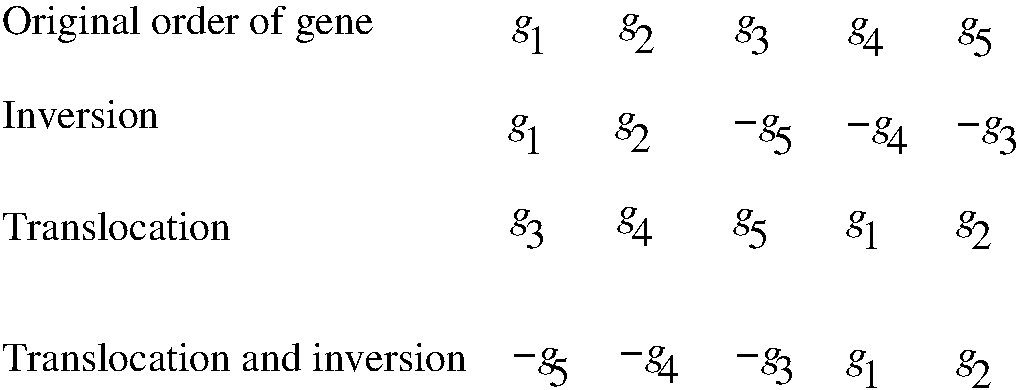
\includegraphics[width=0.6\textwidth]{figures/genomeRearrangement.pdf}
    		\end{center}
    		 \caption{Examples of gene rearrangements: inversions and translocations.}
		 \label{fig:genomeRearrangement}
		\end{figure}

		\begin{figure}[!htbp]
		\begin{center}
        		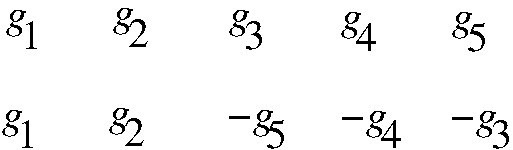
\includegraphics[width=0.4\textwidth]{figures/breakpointDis.pdf}
      		\end{center}
		  \caption{Rearrangement calculations between chromosomal or genomic data of six genes $g_1, \ldots, g_6$,
                 	 where the rearrangement events are detected as either two breakpoints $(g_2, g_3), (g_5, g_6)$
                   or a single inversion $(g_1, g_2, g_3)$.}
                   \label{fig:distance}
		\end{figure}
		
	\begin{description}
            
            	\argumentdefinition{med\_approx}{\obligatory{\poybool}}
                        {Approximates chromosome medians using a fixed-states
                        approach. This is most useful to accelerating tree
                        building and searching operations for large chromosomal
                        data sets. The boolean value \texttt{true} applies the
                        fixed-states optimization. The default value is
                        \texttt{false}.}
                        {medapprox}
                        
                        \argumentdefinition{locus\_breakpoint}{\obligatory{\poyint}}
                        {Calculates the breakpoint distance \cite{blanchetteetal1997}
                        between two pairs of chromosomes given the cost for rearrangement
                        specified by an integer value.  The breakpoint distance calculation considers
                        a chromosome or genome $G = (x_1, \ldots, x_n)$of $n$ gene, wherein each
                        gene appears exactly once and its orientation is either positve or negative.  Gene
                        orders are altered by gene rearrangement operations: gene inversion, gene translocation,
                        gene inversion and translocation (see Figure \ref{fig:genomeRearrangement}).  
                        The breakpoint distance takes into account rearrangements but not inversions.
                        Given $G$ and $G'$, a pair of genes $(g_i, g_j)$ is a breakpoint if $(g_i, g_j)$ occur 
                        consecutively in $G$ but neither $(g_i, g_j)$ nor $(-g_j, -g_i)$ occur
                        consectively in $G'$  \cite{sankoffandblanchette1998}.  The breakpoint distance between $G$
		     and $G^\prime$ is the number of breakpoints between them.  Figure \ref{fig:distance} 
                        shows two breakpoints between $G$ and $G^\prime$. The breakpoint can be calculated 
                        easily in linear time.  This argument \emph{cannot} be used in
                        conjunction with \poyargument{inversion}. The default
                        value of \poyargument{locus\_breakpoint} is \texttt{10}.} 
                        {locusbreakpoint} 
                        
                        \argumentdefinition{locus\_inversion}{\obligatory{\poyint}}
                        {Calculates the inversion distance~\cite{hanenhalliandpevzner1995}
                        between two chromosome segments given the cost for inversion
                        specified by the integer value. The inversion distance
                        takes in consideration rearrangements and
                        inversions. Given $G$ and $G^\prime$, the inversion distance between
                        them is the number of inversions to convert chromosome or genome $G$ 
                        into $G^\prime$ \cite{hanenhalliandpevzner1995}. Figure \ref{fig:distance} shows one inversion  
                        between $G$ and $G^\prime$. The inversion can be calculated in linear time.
                        The breakpoint distance is normally larger than inversion distance.
                        This argument \emph{cannot} be used in conjunction with \poyargument{breakpoint}.} 
                        {locusinversion}  

		     \argumentdefinition{locus\_indel}{\obligatory{(\poyint, \poyfloat)}} 
                        {Specifies the cost for insertion/deletion of a
                        chromosome segment. The integer value sets the gap opening
                        cost ($o$), whereas the float value sets the gap extension
                        cost ($e$).  The indel cost for a fragment of length $l$ is
                        specified by the following formula:
                       $o + l \times e$. The default values are $o=10, e=1.0$.}
                        {locusindel}

		     \argumentdefinition{min\_seed\_length}{\obligatory{\poyint}}
                        {Specifies the minimum length of identical (invariant,
                        completely conserved) contiguous sequence fragments
                        during comparison between two chromosomes. The integer
                        value of \poyargument{min\_seed\_length} is the number of
                        nucleotides. Correct identification of such fragments
                        facilitates detecting chromosome rearrangement events and
                        accelerates other operations (such as tree building and
                        swapping). However, if \poyargument{min\_seed\_length} value
                        is set too low (detecting many short fragments) or
                        too high (such that no identical fragments are detected)
                        the time required for subsequent searching procedures
                        may significantly increase. The optimal \poyargument{min\_seed\_length} 
                        value depends on the specifics of  a given dataset (see Figure \ref{fig:chrom}).
                        The default value of \poyargument{min\_seed\_length} is \texttt{9}.}
                        {minseedlength}

                          \argumentdefinition{min\_loci\_len}{\obligatory{\poyint}}
                          {Creates a pairwise alignment between two chromosomes to
                          detect conserved areas (``blocks''). However, only blocks of
                          lengths (in number of nucleotides) greater or equal to the specified \poyargument{min\_loci\_len}
                          value are considered as hypothetically
                          homologous blocks and used as anchors to divide chromosomes into
                          fragments. Thus, increasing the value of \poyargument{min\_loci\_len} decreases
                           the chance of inferring small-size rearrangements (see Figure \ref{fig:chrom}). 
                           The default value is \texttt{100}.} 
                           {minlocilen}
                           
                           \argumentdefinition{min\_rearrangement\_len}{\obligatory{\poyint}} 
                            {Two seeds are said to be \emph{non-rearranged}, 
               	           if their distance is less than the predefined threshold value set
	                    for \poyargument{min\_rearrangement\_len}.  In other words, it is unlikely 
	                    that rearrangement operations can occur between two non-rearranged seeds
	                    if they are connected (see Figure \ref{fig:chrom}).
	                    The default value is \texttt{100}}
                             {minrearrangementlen}

 			\begin{figure} [!htbp]
   		 	\begin{center}
        			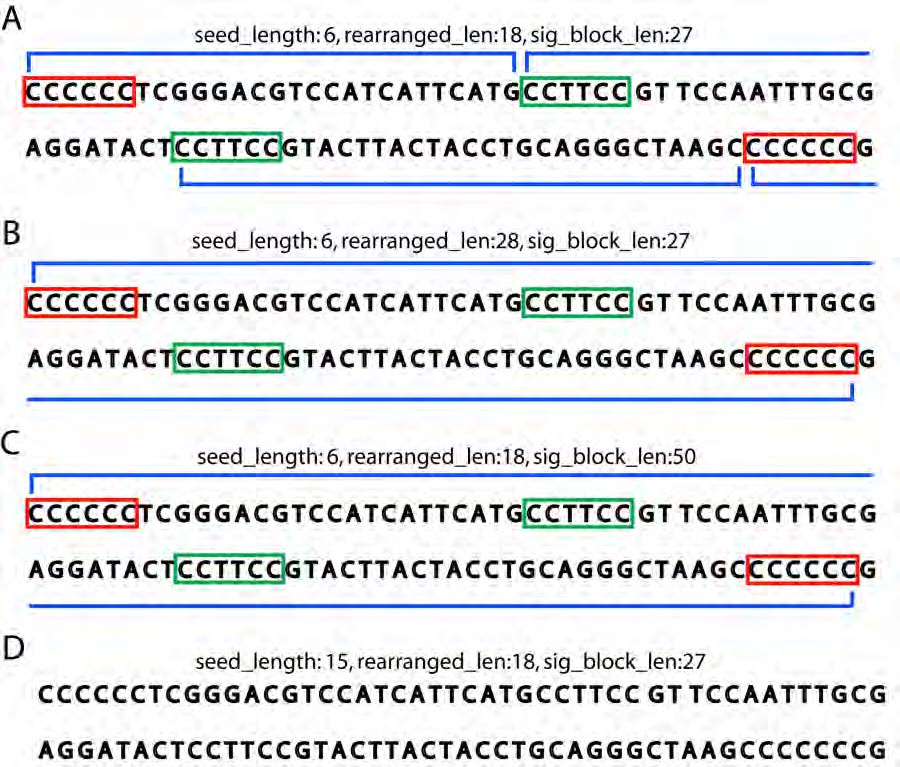
\includegraphics[width=0.8\textwidth]{figures/chromfig1.pdf}
    			\end{center}
    			\caption{The effect of dynamic parameter arguments (\poyargument{seed\_length, min\_rearrangement\_len}, 
			and \poyargument{min\_loci\_len}) on determining homologous blocks in unannotated chromosomal sequences.
			 \emph{Case A} allows for rearrangements between the short homologous blocks within the 				     
			blue brackets constructed upon six nucleotide seeds (red and green), \emph{Case B} 
			restricts rearrangement between seeds that are less than \texttt{28} nucleotides apart.
			 \emph{Case C} restricts rearrangement by requiring homologous blocks at least \texttt{50} nucleotides
			  in length. \emph{Case D} restricts recognition of homology between sequences by setting seed length
			   of conserved seeds at \texttt{15}.}
    		\label{fig:chrom}
		\end{figure}

                       \argumentdefinition{chrom\_breakpoint}{\obligatory{\poyint}} 
      		     {Calculates the breakpoint distance~\cite{blanchetteetal1997}
                        between two sequences of multiple chromosomes given the cost for
                        rearrangement specified by an integer value. The breakpoint distance
                        takes into account locus rearrangements between non-homologous
                        chromosomes (translocations) but not inversions. For further discussion on 
                        how breakpoint distance is calculated see the argument \poyargument{locus\_breakpoint}.  
                        The default value of \poyargument{chrom\_breakpoint} is \texttt{100}.} 
                        {chrombreakpoint}

       
                   \begin{statement}
  		Note that the arguments \poyargument{locus\_breakpoint} and \poyargument {chrom\_breakpoint} cannot be used
		simultaneously with the arguments \poyargument{locus\_inversion} and \poyargument{chrom\_inversion}
		as they designate \emph{alternative} methods of calculating distance between two chromosomes.
		If both arguments are specified, the latter will be executed. The order of other arguments of
		\poyargument{dynamic\_pam} is arbitrary. 
		\end{statement}

		     \argumentdefinition{chrom\_hom}{\obligatory{(\poyfloat)}}
                       {Specifies the lower limit of distance between two chromosomes
                        beyond which the chromosomes are not considered to be
                        homologous. The default value of \poyargument{chrom\_hom}
                        is \texttt{0.75}.}
                        {chromhom}
                        
                         \argumentdefinition{chrom\_indel}{\obligatory{(\poyint, \poyfloat)}}
                        {Specifies the cost for insertion and deletion of a chromosome in analysis of
                        multiple chromosomes. The integer value sets gap opening
                        cost ($o$), whereas the float value sets gap extension
                        cost ($e$).  The indel cost for a fragment of length $l$ is
                        specified by the following formula:
                       $o + l \times e$. The default values are $o=10, e=1.0$.}
                        {chromindel}
 
 	               \argumentdefinition{circular}{\obligatory{\poybool}} 
                        {Specifies if chromosome is circular (boolean value 
                        \texttt{true}) or linear (boolean value \texttt{false}).
                        The default value of \poyargument{circular} is
                        \texttt{false} (linear chromosome).}
                        {circular}

       		      
		      \argumentdefinition{median}{\obligatory{\poyint}}
                        {Specifies the number alternative locus and chromosome
                        rearrangements of the best cost selected (randomly) for
                        each HTU (hypothetical taxon unit) or median. Limiting the number of rearrangements
                        stored in memory (smaller value of \poyargument{median})
                        is heuristic strategy to accelerate calculations at the
                        expense of thoroughness of the search. By default, only 1
                        rearrangement is retained (the first one found). If more than
                        one rearrangement is specified, the selected number of
                        rearrangements is selected in random order from the pool of
                        all generated rearrangements.}
                        {median}

       
       		     \argumentdefinition{swap\_med}{\obligatory{\poyint}}
                        {Specifies the maximum number of swapping iterations
                        to search for best pairwise alignment of two chromosomes
                        taking into account locus-level rearrangement events. Limiting the number of swapping
                        iterations accelerates the search at the expense of
                        thoroughness. The default value is \texttt{1}.}
                        {swapmed}

       
          \end{description}
	\end{argumentgroup}
	\end{arguments}
	

    \poydefaults{}{If no arguments are given, this command does nothing.}

	\begin{poyexamples} 
		\poyexample{transform((all, tcm:(1,1)))} 
             	{Applies the transformation cost matrix (1,1) to all characters,
             	meaning that substitutions and gaps receive the same weight.}

		\poyexample{transform((all, tcm:"molmatrix"))} 
           	 {Applies the character transformation matrix "molmatrix" to all
            	characters.}
            	
		\poyexample{transform((all, tcm:(1,1)))}{This command
		is equivalent to \poycommand{transform((dynamic, tcm:(1,1)))}.}
		
		\poyexample{transform(tcm:(1,1), gap\_opening:1)}
		{Applies the transformation cost matrix and the gap opening cost
		to all characters. In this example the cost for substitutions is \texttt{1},
		the gap opening cost is \texttt{2} (\texttt{1} set by \poyargument{gap\_opening}
		+ \texttt{1} set by \poyargument{tcm}), and the gap extension cost is \texttt{1}
		(set by \poyargument{tcm}).}
		
		\poyexample{transform(tcm:(2,2), ti:(1,1,1,1,0), td:(1,1,1,1,0))}
		{Assigns to all characters the symmetric transformation cost
		matrix with cost \texttt{2} for every indel and substitution, but for those
		insertions and deletions at the ends of the sequences, the cost
		assigned will only be \texttt{1}.}
		
		\poyexample{transform((static, weightfactor:2))}
            	{This command reweights all the static homology characters
            	by a multiplicative factor of \texttt{2}, while keeping the weighting
            	scheme that has been specified before.}
		
		\poyexample{transform((static, weight:4.2))}{Applies the same
		weight (a float value \texttt{4.2}) to all static homology characters.}
		
		\poyexample{transform((dynamic, weight:4))}{Applies the same
		weight (an integer value \texttt{4}) to all dynamic homology characters.}

        		\poyexample{transform((all, tcm:(1,1)), (names:("gen1",
        		"gen2"), \\ static\_approx), (names:("gen3"), tcm:"molmatrix"))}  
            	{Applies the substitution and indel costs \texttt{1} to all characters, then applies static approximation
            	using that tcm to characters in files \texttt{gen1} and \texttt{gen2}, and for file
            	gen3, it invokes a different transformation cost matrix, contained
            	in the file molmatrix. Beware that the file name should be exactly
            	as it was reported with \poycommand{report(data)}, which differs from the actual
            	file name (\poycommand{report (data)} reports files as fileX:N).}

        		\poyexample{transform((all, tcm:(1,1)), (names:("gen1:3",
        		"gen2:10", \\"gen3:1", "gen4:5"), static\_approx), (names:("gen5", \\
        		"gen6"), tcm:"Molmatrix1"))}
            	{Applies \poyargument{tcm (1,1)} to all characters, then applies
            	static approximation to the sequence data contained in files \texttt{gen1}, \texttt{gen2},
            	\texttt{gen3}, and \texttt{gen4} according to this transformation cost
            	matrix, and applies the custom transformation cost matrix contained in the file
            	\texttt{Molmatrix1} to the sequence data contained in files \texttt{gen5} and
            	\texttt{gen6}.}
         
         		\poyexample{transform(fixed\_states)}
        		 {Transformed all sequence characters into fixed states characters.}
            
          	\poyexample{transform((names:("gen1", "gen4"), fixed\_states))}
           	{Transformed only specified sequence characters (\texttt{gen1} and
           	\texttt{gen4}) into fixed states characters.}
           
           	\poyexample{transform(custom\_to\_breakinv:(circular:true))}
           	{In this example all custom\_alphabet data is transformed into the breakinv data type 
		and is treated as a circular chromosome.}
          
          	\poyexample{transform(seq\_to\_chrom:(locus\_indel:(50, 1.0), min\_seed\_length:15))} 
          	{All applicable (\emph{i.e.} sequence) data are transformed into chromosome
          	data with the minimum length of identical contiguous sequence fragments which form
	          the seeds of homologous blocks set at  \texttt{15} nucleotides and the locus-level gap
	         opening cost is set at \texttt{50} with a gap extension cost at \texttt{1.0}.}
              
          	\poyexample{transform((all, dynamic\_pam:(locus\_breakpoint:10, min\_rearrangement\_len:60, median:1, circular:false)))} 
             	{This example shows the transformation of chromosomal data using the argument \poyargument{dynamic\_pam}
		to set the locus rearrangement (breakpoint) cost at \texttt{10}, and only strings of \texttt{60} or more nucleotides 
		are considered in determining possible rearrangements between identified seeds.  The chromosome data are
		treated as linear and only a single set of median rearrangements are stored.}
            
	\end{poyexamples}	    

\end{command}


\begin{command}{use}{}

	\syntax{\obligatory{(\poystring)}}

	\begin{poydescription}
         Restores from memory the state of a \poy session (that includes character data,
         selections, trees, all other data and specifications) that had previously been
         saved during the session using the command~\ccross{store}{}. The recalled
         session replaces the current session. The string argument specifies the name
         of the stored state.
         
         In combination with ~\ccross{store}{}, the command \poycommand{use}
         is very useful for exploring alternative  cost regimes and terminal sets
         within a single \poy session.
            
	\end{poydescription}
	
	\begin{poyexamples}
        \poyexample{store("initial\_tcm") \\ transform(tcm:(1,1)) \\ use("initial\_tcm")}
            {The first command, \poycommand{store}, stores the current
            characters and trees under the
            name \texttt{initial\_tcm}. The second command,
            \poycommand{transform}, changes the cost regime of molecular characters,
            effectively changing the data being analyzed. However, the third
            command, \poycommand{use}, recovers the initial state stored under the
            name \texttt{initial\_tcm}.}
    \end{poyexamples}

     \begin{poyalso}
        \cross{store}
        \cross{transform}
    \end{poyalso}

\end{command}

\begin{command}{version}{}

	\syntax{\obligatory{()}}

	\begin{poydescription}
            Reports the \poy version number in the output window of the ncurses
            interface, or to the standard error in the flat interface.
	\end{poydescription}

    \begin{poyexamples}
        \poyexample{version ()}{}
    \end{poyexamples}
\end{command}

\begin{command}{wipe}{}

	\syntax{\obligatory{()}}

	\begin{poydescription}
        Eliminates the data stored in memory (all character data, trees, \emph{etc.}).
	\end{poydescription}

    \begin{poyexamples}
        \poyexample{wipe ()}{}
    \end{poyexamples}
\end{command}
      
